\RequirePackage{currfile} 

\documentclass[compress]{beamer}

\mode<presentation> {

\usetheme{Boadilla}
\usecolortheme{beaver}
\useinnertheme{rectangles}
\setbeamertemplate{navigation symbols}{}

%\setbeamercovered{transparent} % Fait apparaître les animations en grisé (utile pour la conception, mais peut être commenté lors de la remise du document final)

\usefonttheme{serif}

}

\usepackage{graphicx} % Allows including images
\usepackage{booktabs} % Allows the use of \toprule, \midrule and \bottomrule in tables




% Les autres packages utiles  notamment pour le français, les accents ou Python
\usepackage{natbib}         % Pour la bibliographie
\usepackage{url}            % Pour citer les adresses web
\usepackage[T1]{fontenc}    % Encodage des accents
\usepackage[utf8]{inputenc} % Lui aussi
\usepackage{numprint}       % Histoire que les chiffres soient bien

\usepackage{amsmath}        % La base pour les maths
\usepackage{mathrsfs}       % Quelques symboles supplémentaires
\usepackage{amssymb}        % encore des symboles.
\usepackage{amsfonts}       % Des fontes, eg pour \mathbb.

\usepackage{cancel}

\usepackage{siunitx}
\sisetup{
    detect-all,
    output-decimal-marker={,},
    group-minimum-digits = 3,
    group-separator={~},
    number-unit-separator={~},
    inter-unit-product={~}
}

\usepackage{tabularx}

%%%% Pour L'utilisation de C
\usepackage{listings}

\usepackage{minted}

\usepackage{commutative-diagrams}
\usepackage{circuitikz}
% Les macros et raccourcis personnels
% Ce fichier contient toutes les macros que vous pouvez avoir envie de définir 
% si vous les utilisez plusieurs fois dans le document.

\PassOptionsToPackage{svgnames}{color}

% Un environnement pour bien présenter le code informatique
\newenvironment{code}{%
  \begin{mdframed}[linecolor=green,innerrightmargin=30pt,innerleftmargin=30pt,
  backgroundcolor=black!5,
  skipabove=10pt,skipbelow=10pt,roundcorner=5pt,
  splitbottomskip=6pt,splittopskip=12pt]
  }{%
\end{mdframed}
}

% Un raccourci pour composer les unités correctement (en droit)
% Exemple: $v = 10\U{m.s^{-1}}$
\newcommand{\U}[1]{~\mathrm{#1}}

% Les guillemets \ofg{par exemple}
\newcommand{\ofg}[1]{\og{}#1\fg{}}

% Le d des dérivées doit être droit: \frac{\dd x}{\dd t}
\newcommand{\dd}{\text{d}}

% La dérivée temporelle, tellement courante en physique, avec les d droits
\newcommand{\ddt}[1]{\frac{\dd #1}{\dd t}}

% Des parenthèses, crochets et accolades qui s'adaptent automatiquement à la 
% taille de ce qu'il y a dedans
\newcommand{\pa}[1]{\left(#1\right)}
\newcommand{\pac}[1]{\left[#1\right]}
\newcommand{\paa}[1]{\left\{#1\right\}}

% Un raccourci pour écrire une constante
\newcommand{\cte}{\text{C}^{\text{te}}}

% Pour faire des indices en mode texte (comme les énergie potentielles)
\newcommand{\e}[1]{_{\text{#1}}}

% Le produit vectoriel a un nom bizarre:
\newcommand{\vectoriel}{\wedge}


% On définit le titre et l'auteur du document

% L'argument optionnel (entre crochets) donne le titre qui sera mis sur chaque slide
\title[]{La transformée de Fourier appliquée à la compression d'images}
\author[]{Maxence Bellanger : N°15857} % Votre nom
% L'épreuve (car on n'a pas le droit de signaler sa provenance à un concours) (là encore, l'argument optionnel apparaît sur chaque slide)
\institute[]{Épreuve de TIPE}
\date{} 

% On démarre le document proprement dit
\begin{document}

% La page de titre et la table des matières
% Rien d'autre à faire qu'afficher le titre
\begin{frame}
    \titlepage{}
\end{frame}


% La table des matières utilise ce que vous donnez aux commandes \section et 
% \subsection tout au long de la présentation.
\begin{frame}
    \frametitle{Plan de l'exposé} 
    \tableofcontents 
\end{frame}


%\begin{frame}{Explication du problème et lien avec la ville}{Un petit calcul}
%    \begin{itemize}
%        \item <1-> Un pixel est un élément de \([\![0;255]\!]^3\) il nécessite donc \(3\) bits pour être stocké.
%        \item <2-> Une image de haute définition (HD) est composée de \(1280\times720\) pixels.
%        \item <3-> Une caméra enregistre à environ 30 images par secondes.
%        \item <4-> Une caméra de surveillance qui enregistrerait pendant 1 journée produirait donc \(30\times24\times60\times60 = 2592000\) images.
%        \item <5-> On obtiendrait donc un fichier de  \(7^{12}\) bits soit \(7\U{To}\). 
%    
%    \end{itemize}
%\end{frame}

\begin{frame}{Explication du problème et lien avec la ville}{Un petit calcul}
    \begin{itemize}
        \item <1-> Un pixel = \textbf{3 octets}
        \item <2-> Une image en HD = \textbf{921 600 pixels}
        \item <3-> Une seconde de vidéo = \textbf{30 images}
        \item <4-> Un enregistrement de surveillance de une journée = \textbf{7 To} 
        \item <5-> La taille d'un disque dur moyen = \textbf{1 To}
    \end{itemize}
\end{frame}


% Première partie : Comment compresser
\section{Comment compresser une image}

%%%%%%%%%%%%%%%%%%%%%%%%%%%%%%%%%%%%%%%%%%%%%%%%
% Première diapo
%%%%%%%%%%%%%%%%%%%%%%%%%%%%%%%%%%%%%%%%%%%%%%%%
\begin{frame}{Comment compresser une image}{Une première approche \dots}
    \begin{align*}
        \underbrace{111\dots111}_{\text{100 fois}} \longrightarrow \textrm{100*1} 
    \end{align*} 

    \begin{center}
        On gagne un facteur \textbf{20} !
    \end{center}
\end{frame}

%%%%%%%%%%%%%%%%%%%%%%%%%%%%%%%%%%%%%%%%%%%%%%%%
% Deuxième diapo
%%%%%%%%%%%%%%%%%%%%%%%%%%%%%%%%%%%%%%%%%%%%%%%%
\begin{frame}{Comment compresser une image}{\dots peu satisfaisante.}
    \begin{itemize}
        \item \(\displaystyle\sum_{k=0}^{N-x-1}2^k = 2^{N - x} - 1\) fichiers de taille strictement inférieur à \(N-x\) bits.
        \item \(2^N\) fichiers de taille $N$ bits.
    \end{itemize}
    On a une proportion de \(\frac{2^{N-10} - 1}{2^N} < \frac{1}{2^{10}} = \mathbf{\frac{1}{1024}}\) fichiers compressibles d'au moins 10 bits
\end{frame}

%%%%%%%%%%%%%%%%%%%%%%%%%%%%%%%%%%%%%%%%%%%%%%%%
% Troisième diapo
%%%%%%%%%%%%%%%%%%%%%%%%%%%%%%%%%%%%%%%%%%%%%%%%
%\begin{frame}{Comment compresser une image}{Compression avec pertes}
%    \begin{codi}
%        \obj{A &&&&&& B \\
%             C &&&&&& D\\};
%
%        \mor :[bend left] A transformation :-> B;
%        \mor : B quantification :-> C;
%        \mor :[bend right] C compression :-> D;
%    \end{codi}
%\end{frame}

\begin{frame}{Comment compresser une image}{Compression avec pertes}
    \begin{figure}[!ht]
        \centering
        \resizebox{0.7\textwidth}{!}{%
        \begin{circuitikz}
        \tikzstyle{every node}=[font=\Huge, line width = 40]
        \draw[line width = 3.0] (0,18) rectangle  node {Image} (5,12);
        \draw[line width = 3.0, -Stealth] (5,15) -- (7,15);
        \draw[line width = 3.0] (7,18) rectangle  node[align = center] {Image\\transformée} (12,12);
        \draw[line width = 3.0, -Stealth] (12,15) -- (14,15);
        \draw[line width = 3.0] (14,18) rectangle  node[align = center] {Image\\quantifiée} (19,12);
        \draw[line width = 3.0, -Stealth] (19,15) -- (21,15);
        \draw[line width = 3.0] (21,18) rectangle  node[align = center] {Image\\compressée} (26,12);
        \end{circuitikz}
        }%
        \caption{Schéma d'un algorithme de compression d'image}
    \end{figure}
\end{frame}

% Deuxième partie : Introduction à la TF
%Titre
\section{La transformée de Fourier}

%%%%%%%%%%%%%%%%%%%%%%%%%%%%%%%%%%%%%%%%%%%%%%%%
% Première diapo
%%%%%%%%%%%%%%%%%%%%%%%%%%%%%%%%%%%%%%%%%%%%%%%%
\begin{frame}{La transformée de Fourier}{}
    \begin{block}{Definition}
        La transformée de Fourier est un opérateur, qui permet de transformer un signal sous forme temporelle en signal sous forme fréquentielle: 
         \[ \forall f \in L^1 \, \forall x \in \mathbb{R} \; \mathcal{F}(f)(x) = \int_{-\infty}^{+\infty} f(t)e^{-2i\pi xt}\mathrm{d}t\]
    \end{block}
\end{frame}

%%%%%%%%%%%%%%%%%%%%%%%%%%%%%%%%%%%%%%%%%%%%%%%%
% Deuxième diapo
%%%%%%%%%%%%%%%%%%%%%%%%%%%%%%%%%%%%%%%%%%%%%%%%
\begin{frame}{La transformée de Fourier}{Représentation fréquentielle d'une image}
	\begin{itemize}
		\item <1-> \textbf{Basses fréquences = informations importantes} de l'image : dégradés doux,  aplat.
		\item <2-> \textbf{Hautes fréquences = détails} : contours, bruits.
		\item <3-> Les \textbf{hautes fréquences} seront \textbf{atténuées} lors de la \textbf{compression}, pour que les changements soient peu perceptibles. 
	\end{itemize}
\end{frame}

%%%%%%%%%%%%%%%%%%%%%%%%%%%%%%%%%%%%%%%%%%%%%%%%
% Troisième diapo
%%%%%%%%%%%%%%%%%%%%%%%%%%%%%%%%%%%%%%%%%%%%%%%%
\begin{frame}{La transformée de Fourier}{Représentation fréquentielle d'une image}
	\begin{figure}
		\begin{tabular}{ c c }
			
\includegraphics[scale=1.2]{images/TF/exemples_diapo_2/blason-cachan.png} &
			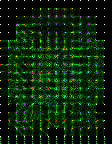
\includegraphics[scale=1.2]{images/TF/exemples_diapo_2/blason-cachan_tf_couleur.png}
		\end{tabular}
		\caption{La transformée de Fourier d'une image}
	\end{figure}
\end{frame}


%%%%%%%%%%%%%%%%%%%%%%%%%%%%%%%%%%%%%%%%%%%%%%%%
% Quatrième diapo
%%%%%%%%%%%%%%%%%%%%%%%%%%%%%%%%%%%%%%%%%%%%%%%%
\begin{frame}{La transformée de Fourier}{Comment calculer la transformée de Fourier d'une image}
	\begin{block}{Transformée de Fourier discrète}
		La transformée de Fourier est une application linéaire de \(\mathbb{C}^n$ dans $\mathbb{C}^n\)
		Soit \(X\in\mathbb{C}^n\) \\
		Le vecteur transformé s'exprime \(\widehat{X} = AX\) avec \(A = {\left(\exp\left(2\mathbf{i}\pi\frac{kl}{n}\right)\right)}_{\substack{0 \leqslant k \leqslant n-1,\\ 0 \leqslant l \leqslant n-1}}\)
	\end{block}
\end{frame}

%%%%%%%%%%%%%%%%%%%%%%%%%%%%%%%%%%%%%%%%%%%%%%%%
% Cinquième diapo
%%%%%%%%%%%%%%%%%%%%%%%%%%%%%%%%%%%%%%%%%%%%%%%%
\begin{frame}{La transformée de Fourier}{Comment calculer la transformée de Fourier d'une image}
	\begin{align*}
		{
		M = 
		\begin{pmatrix}
				x_{0,0} \dots x_{0,n-1} \\
				\vdots \phantom{x_{0} \dots x_{0}} \vdots\\ 
				x_{n-1,0} \dots x_{n-1,n-1} \\
		\end{pmatrix}
		}
		\longrightarrow
		{
		 	\begin{pmatrix}
				x_{0,0}\\
				\vdots\\
				x_{0,n-1}\\
				\vdots\\
				x_{n-1,n-1}
			\end{pmatrix}
		}
		= X
	\end{align*}
\end{frame}

%%%%%%%%%%%%%%%%%%%%%%%%%%%%%%%%%%%%%%%%%%%%%%%%
% Sixième diapo
%%%%%%%%%%%%%%%%%%%%%%%%%%%%%%%%%%%%%%%%%%%%%%%%
\begin{frame}{La transformée de Fourier}{Comment calculer la transformée de Fourier d'une image}
	\begin{block}{Algorithme naïf}
		Soit \(X \in \mathbb{C}^{n\times m}\)\\
		\begin{itemize}
			\item <2-> \(X = (x_{i,j})_{\substack{0 \leqslant k \leqslant n-1,\\ 0 \leqslant l \leqslant m-1}}\)
			\item <3-> \(A = \left(\frac{1}{\sqrt{nm}}\exp{\left(2\mathbf{i}\pi\left(\frac{ik}{n}+\frac{jl}{m}\right)\right)}\right)_{\substack{0 \leqslant i,k \leqslant n-1,\\ 0 \leqslant j,l \leqslant m-1}}\)
		\end{itemize}
		
		\onslide<4->{D'où le vecteur transformé :
		\[\widehat{X}_{i,j} = [AX]_{i,j} = \frac{1}{\sqrt{nm}}\sum_{k=0}^{n}\sum_{l=0}^{m-1} x_{k,l}e^{\left(2\mathbf{i}\pi\left(\frac{ik}{n}+\frac{kl}{m}\right)\right)}\]
		}
	\onslide<5-> On obtient donc un algorithme en \(\mathcal{O}(N^2)\) où \(N=n\times m\) est la taille de l'image.
	\end{block}
\end{frame}

%%%%%%%%%%%%%%%%%%%%%%%%%%%%%%%%%%%%%%%%%%%%%%%%
% Septième diapo
%%%%%%%%%%%%%%%%%%%%%%%%%%%%%%%%%%%%%%%%%%%%%%%%
\begin{frame}{La transformée de Fourier}{De meilleurs algorithmes}
	\begin{block}{Utiliser la séparabilité}
		\onslide<2->{On peut réécrire le calcul précédent : 
		\[\widehat{X}_{i,j} = [AX]_{i,j} = \frac{1}{\sqrt{n}}\sum_{k=0}^{n-1} e^{\left(2\mathbf{i}\pi\left(\frac{ik}{n}\right)\right)} \frac{1}{\sqrt{m}}\sum_{l=0}^{n-1} x_{k,l}e^{\left(2\mathbf{i}\pi\left(\frac{jl}{m}\right)\right)}\]
		}
		\onslide<3-> On voit apparaître deux transformations unidimensionnelles successives, sur les lignes, puis les colonnes.\\

		\onslide<4->{Dans le cas où \(n = m\), le calcul du vecteur transformé devient : 

		\[\widehat{M} = AMA^t, \textrm{où} \, A = {\left(\frac{1}{\sqrt{n}}\exp\left(2\mathbf{i}\pi\frac{kl}{n}\right)\right)}_{\substack{0 \leqslant k \leqslant n-1,\\ 0 \leqslant l \leqslant n-1}}\]
		}
		\onslide<5->On obtient finalemenent un algorithme en \(\mathcal{O}(N)\) où \(N=n\times m\) est la taille de l'image.
	\end{block}
\end{frame}	

%%%%%%%%%%%%%%%%%%%%%%%%%%%%%%%%%%%%%%%%%%%%%%%%
% Huitième diapo
%%%%%%%%%%%%%%%%%%%%%%%%%%%%%%%%%%%%%%%%%%%%%%%%
\begin{frame}{La transformée de Fourier}{La transformée en cosinus discrète}
	
	\onslide<1->{
	\begin{block}{Inconvénients de la transformée de Fourier}
		\begin{itemize}
			\item <2-> Coefficients complexes
			\item <3-> Décroissance des coefficients vers le centre de l'image \(\rightarrow\) suppression de coefficients importants :
			contradictions avec le Système Visuel Humain.
		\end{itemize}
	\end{block}
	}
	\onslide<4->{
	\begin{block}{Une solution : la transformée en cosinus discrète}
		\begin{itemize}
			\item <5-> Opération basés sur la TF donc mêmes avantages
			\item <6-> Règle les problèmes énumérés précédement
			\item <7-> Décroissance des coefficients vers les hautes fréquences \(\rightarrow\) en accord avec le Système Visuel Humain 
		\end{itemize}
	\end{block}
	}

\end{frame}

%%%%%%%%%%%%%%%%%%%%%%%%%%%%%%%%%%%%%%%%%%%%%%%%
% Neuvième diapo
%%%%%%%%%%%%%%%%%%%%%%%%%%%%%%%%%%%%%%%%%%%%%%%%
\begin{frame}{La transformée de Fourier}{Comparaison entre la TF et la TCD}
	\begin{figure}
		\begin{tabular}{ c c c}
			
\includegraphics[scale=13]{images/TF/comparaison_tf_tcd/diapo_tf_img.png} &
			
\includegraphics[scale=13]{images/TF/comparaison_tf_tcd/diapo.png} &
			
\includegraphics[scale=13]{images/TF/comparaison_tf_tcd/diapo_tcd_img.png}
		\end{tabular}
		\caption{À gauche TF; Au milieu image de base; À droite TCD}
	\end{figure}
\end{frame}

% Troisième partie : Algorithme de compression
\section{Algorithmes de compression}
%%%%%%%%%%%%%%%%%%%%%%%%%%%%%%%%%%%%%%%%%%%%%%%%
% Première diapo
%%%%%%%%%%%%%%%%%%%%%%%%%%%%%%%%%%%%%%%%%%%%%%%%
\begin{frame}{Algorithmes de compression}{Méthodes de quantification}
   \onslide<1-> \begin{block}{Différentes méthodes envisagées :}
        \begin{itemize}
            \item <2-> Selection par seuil
            \item <3-> Selection par zone
            \item <4-> Matrice de Quantification
        \end{itemize}
    \end{block} 
\end{frame}

%%%%%%%%%%%%%%%%%%%%%%%%%%%%%%%%%%%%%%%%%%%%%%%%
%% Deuxième diapo
%%%%%%%%%%%%%%%%%%%%%%%%%%%%%%%%%%%%%%%%%%%%%%%%%
%\begin{frame}{Algorithme de compression}{Exemples : Selection par zone}
%    On garde uniquement les coefficients au dessus d'une certaines zones
%
%    \begin{block}{Selection par zone}
%        \scalebox{0.8}[1.5]{
%            \begin{tabular}{|c|c|c|c|c|c|c|c|}
%                \hline 1722 & -108 & 3 & -2 & -4 & 0 & 0 & -2  \\
%                \hline 76 & 12 & -25 & -1 & 0 & 0 & -2 & 1 \\ 
%                \hline 12 & -4 & 4 & -1 & -2 & -1 & 1 & 0 \\ 
%                \hline 0 & 1 & 2 & -2 & 1 & -1 & 0 & 1 \\ 
%                \hline -4 & -1 & 0 & 1 & 0 & 0 & 1 & 0 \\ 
%                \hline -3 & 6 & -1 & -1 & 0 & 0 & -1 & 1 \\ 
%                \hline 1 & -3 & 0 & 1 & 0 & 0 & 0 & -1 \\ 
%                \hline 0 & 1 & 0 & -1 & 0 & 0 & 0 & 1 \\\hline
%            \end{tabular}
%            \(\rightarrow\)
%            \begin{tabular}{|c|c|c|c|c|c|c|c|}
%                \hline 1722 & -108 & 3 & -2 & -4 & 0 & 0 & -2  \\
%                \hline 76 & 12 & -25 & -1 & 0 & 0 & -2 & 1 \\ 
%                \hline 12 & -4 & 4 & -1 & -2 & -1 & 1 & 0 \\ 
%                \hline 0 & 1 & 2 & 0 & 0 & 0 & 0 & 0 \\ 
%                \hline -4 & -1 & 0 & 0 & 0 & 0 & 0 & 0 \\ 
%                \hline -3 & 6 & -1 & 0 & 0 & 0 & 0 & 0 \\ 
%                \hline 1 & -3 & 0 & 0 & 0 & 0 & 0 & 0 \\ 
%                \hline 0 & 1 & 0 & 0 & 0 & 0 & 0 & 0 \\\hline
%            \end{tabular}
%        }
%    \end{block}
%\end{frame}
%    
%%%%%%%%%%%%%%%%%%%%%%%%%%%%%%%%%%%%%%%%%%%%%%%%%
%% Troisième diapo
%%%%%%%%%%%%%%%%%%%%%%%%%%%%%%%%%%%%%%%%%%%%%%%%%
%\begin{frame}{Algorithme de compression}{Exemples : Selection par seuil}
%    On garde uniquement les coefficients au dessus d'un certain seuil
%
%    Mettre des exemples
%    \begin{align*}
%        \onslide<1->{
%            \begin{pmatrix}
%                1 & 2 & 3 & 4 & 5 & 6 & 7 & 8 & 9 \\
%                1 & 2 & 3 & 4 & 5 & 6 & 7 & 8 & 9 \\
%                1 & 2 & 3 & 4 & 5 & 6 & 7 & 8 & 9 \\
%                1 & 2 & 3 & 4 & 5 & 6 & 7 & 8 & 9 \\
%                1 & 2 & 3 & 4 & 5 & 6 & 7 & 8 & 9 \\
%                1 & 2 & 3 & 4 & 5 & 6 & 7 & 8 & 9 \\
%                1 & 2 & 3 & 4 & 5 & 6 & 7 & 8 & 9 \\
%                1 & 2 & 3 & 4 & 5 & 6 & 7 & 8 & 9 \\
%            \end{pmatrix}
%        }
%        \onslide<2->{\longrightarrow}
%        \onslide<3->{
%            \begin{pmatrix}
%                1 & 2 & 3 & 4 & 5 & 6 & 7 & 8 & 9 \\
%                1 & 2 & 3 & 4 & 5 & 6 & 7 & 8 & 9 \\
%                1 & 2 & 3 & 4 & 5 & 6 & 7 & 8 & 9 \\
%                1 & 2 & 3 & 4 & 5 & 6 & 7 & 8 & 9 \\
%                1 & 2 & 3 & 4 & 5 & 6 & 7 & 8 & 9 \\
%                1 & 2 & 3 & 4 & 5 & 6 & 7 & 8 & 9 \\
%                1 & 2 & 3 & 4 & 5 & 6 & 7 & 8 & 9 \\
%                1 & 2 & 3 & 4 & 5 & 6 & 7 & 8 & 9 \\
%            \end{pmatrix}
%        }
%    \end{align*}
%\end{frame}
%
%

%%%%%%%%%%%%%%%%%%%%%%%%%%%%%%%%%%%%%%%%%%%%%%%%
% Quatrième diapo
%%%%%%%%%%%%%%%%%%%%%%%%%%%%%%%%%%%%%%%%%%%%%%%%
\begin{frame}{Algorithmes de compression}{Exemples : Matrice de Quantification}
    \begin{block}{Matrice de quantification}
        A partir d'une matrice de quantification Q.
        \newline\newline
        \onslide<2-> L'opération quantification est la suivante : \\
        \onslide<3-> \[\widehat{A}_{i,j} = \left\lfloor\frac{A_{i,j}}{Q_{i,j}}\right\rfloor\] \\

        \onslide<4-> La déquantification s'écrit de la manière suivante : \\
        \[A_{i,j} \approx \widehat{A}_{i,j}\times Q_{i,j} \]
    \end{block}
\end{frame}

%%%%%%%%%%%%%%%%%%%%%%%%%%%%%%%%%%%%%%%%%%%%%%%%
% Cinquième diapo
%%%%%%%%%%%%%%%%%%%%%%%%%%%%%%%%%%%%%%%%%%%%%%%%
%\begin{frame}{Algorithme de compression}{Exemples : Matrice de Quantification}
%
%\end{frame}

%%%%%%%%%%%%%%%%%%%%%%%%%%%%%%%%%%%%%%%%%%%%%%%%
% Sixième diapo
%%%%%%%%%%%%%%%%%%%%%%%%%%%%%%%%%%%%%%%%%%%%%%%%
\begin{frame}{Algorithmes de compression}{Algorithme formel}
    \onslide<1->
    \begin{block}{Algorithme de compression}
        \begin{itemize}
            \item <1-> Tranformation des couleurs en YCbCr
            \item <2-> Tranformée en Cosinus discrète
            \item <3-> Quantification des plans de Luminances et Chrominances
            \item <4-> Compression sans pertes
        \end{itemize}    
    \end{block}
    \onslide<5->
    \begin{block}{Algorithme de décompression}
        \begin{itemize}
            \item Decompression
            \item Déquantification
            \item Tranformée inverse
            \item Tranformation des couleurs en RGB
        \end{itemize}
    \end{block}
\end{frame}

%%%%%%%%%%%%%%%%%%%%%%%%%%%%%%%%%%%%%%%%%%%%%%%%
% Septième diapo
%%%%%%%%%%%%%%%%%%%%%%%%%%%%%%%%%%%%%%%%%%%%%%%%

%Quatrième partie : Evaluation de la qualité
\section{Evaluation de la qualité de la compression}
%%%%%%%%%%%%%%%%%%%%%%%%%%%%%%%%%%%%%%%%%%%%%%%%
% Première diapo
%%%%%%%%%%%%%%%%%%%%%%%%%%%%%%%%%%%%%%%%%%%%%%%%
\begin{frame}{Evaluation de la qualité de la compression}{Critère de qualité}
    \begin{block}{EQM}
        Soient \(A, B\) deux images de dimension \(N \times M\). On a :
        \[EQM(A, B) = \frac{1}{N\times M} \sum^{N-1}_{i=0}\sum^{M-1}_{j=0}(A_{i,j} - B_{i,j})^2 \] 

        De plus la transformée en cosinus discrète étant une isométrie il suffit de comparer les images transformées
    \end{block}
    
\end{frame}
    
%%%%%%%%%%%%%%%%%%%%%%%%%%%%%%%%%%%%%%%%%%%%%%%%
% Troisième diapo
%%%%%%%%%%%%%%%%%%%%%%%%%%%%%%%%%%%%%%%%%%%%%%%%
\begin{frame}{Evaluation de la qualité de la compression}{Résultats}
    \begin{figure}
		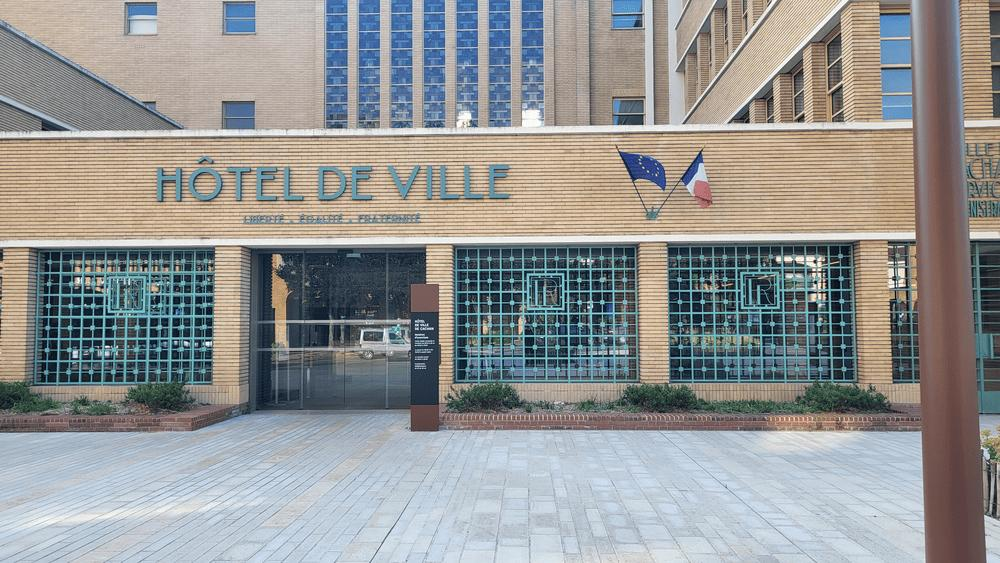
\includegraphics[scale=0.32]{images/resultats_compression/mairie_petit.jpeg}
    \caption{Pas  de compression | Taille de l'image : 1.7 Mo}
    \end{figure}
\end{frame}

\begin{frame}{Evaluation de la qualité de la compression}{Résultats}
  \begin{figure}
  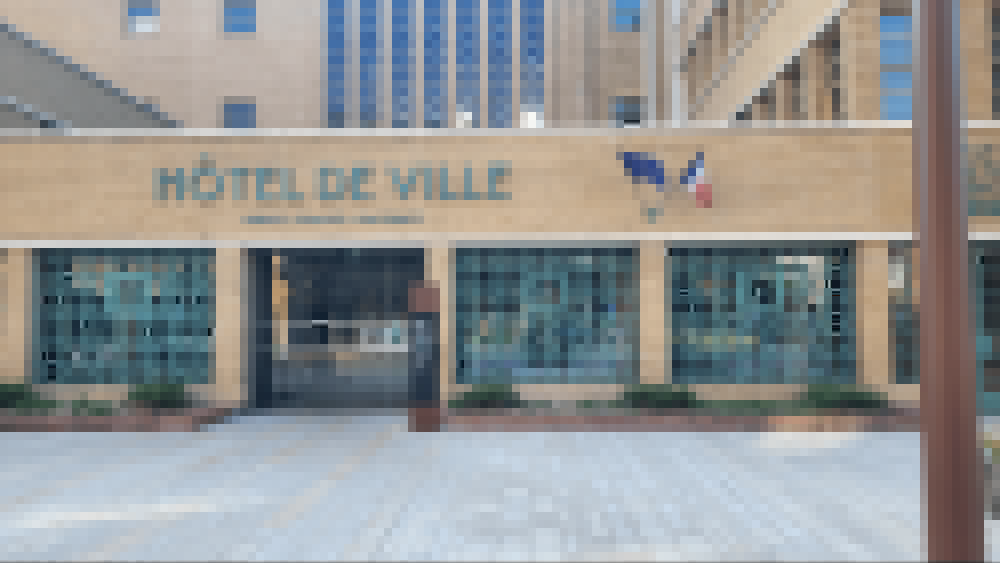
\includegraphics[scale=0.32]{images/resultats_compression/mairie_petit_tcd_seuil_finale.png} 
  \caption{Selection par seuil | Taille de l'image : 67.1 Ko}
  \end{figure}
\end{frame}


\begin{frame}{Evaluation de la qualité de la compression}{Résultats}
    \begin{figure}
		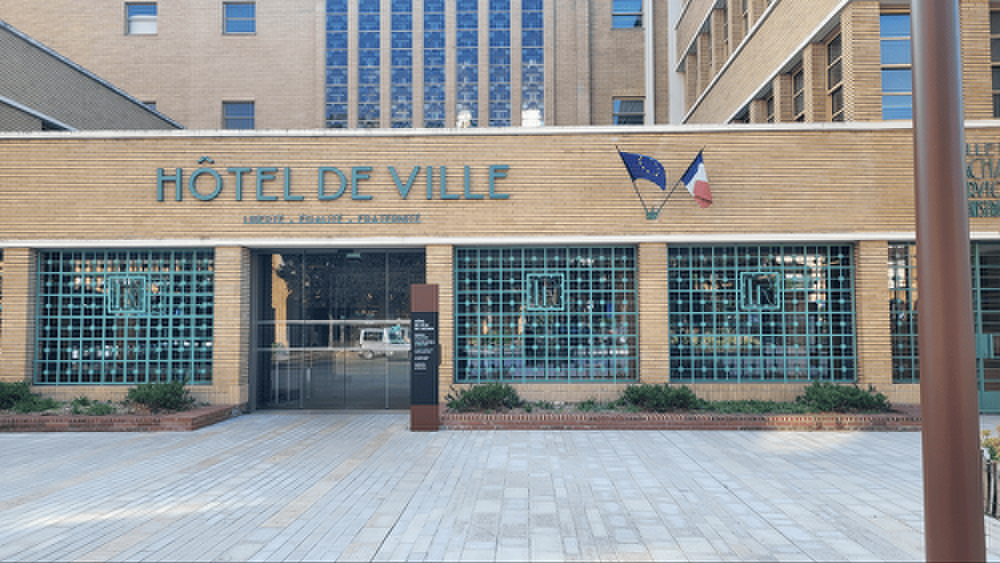
\includegraphics[scale=0.32]{images/resultats_compression/mairie_petit_tcd_zone_finale.png}
    \caption{Selection par zone | Taille de l'image : 667.2 Ko}
    \end{figure}
\end{frame}

\begin{frame}{Evaluation de la qualité de la compression}{Résultats}
    \begin{figure}
		
\includegraphics[scale=0.32]{images/resultats_compression/mairie_petit_tcd_matrice_finale.png} 
    \caption{Matrice de quantification | Taille de l'image : 884.3 Ko}
    \end{figure}
\end{frame}

\begin{frame}{Evaluation de la qualité de la compression}{Résultats}
  \begin{figure}
  
\includegraphics[scale=0.32]{images/resultats_compression/mairie_petit_tf_matrice_finale.png} 
  \caption{Matrice de quantification (avec TF) | Taille de l'image : }
  \end{figure}
\end{frame}

\begin{frame}{Evaluation de la qualité de la compression}{Résultats}
  \begin{block}{Qualité de la compression par seuil}
    \begin{itemize}
      \item EQM pour la TF : 875.378565 
      \item EQM pour la TCD : 873.492274 
    \end{itemize}  
  \end{block}
  \begin{block}{ Qualité de la compression par zone}
    \begin{itemize}
      \item EQM pour la TF : 540.464145 
      \item EQM pour la TCD : 320.759758
    \end{itemize}  
  \end{block}
  \begin{block}{Qualité de la compression par matrice de quantification}
    \begin{itemize}
      \item EQM pour la TF : 11390.811799 
      \item EQM pour la TCD : 11249.098810 
    \end{itemize}  
  \end{block}
\end{frame}

% Conclusion
\input{diapos/05_conclusion.tex}

%Annexe
\section{Annexe}

\begin{frame}{Annexe}{Transformation de Fourier inverse}
    \begin{block}{Avec séparabilité}
        \[M = A^{-1}\widehat{M}(A^{-1})^t, \textrm{où} \; A^{-1} = {\left(\frac{1}{\sqrt{n}}\exp\left(-2\mathbf{i}\pi\frac{kl}{n}\right)\right)}_{\substack{0 \leqslant k \leqslant n-1,\\ 0 \leqslant l \leqslant n-1}}\]
    \end{block}
\end{frame}

\begin{frame}{Annexe}{Preuve que la matrice de la transformée de Fourier est unitaire}
    \footnotesize{
        \[{\textrm{On note : } A = \left(\frac{1}{\sqrt{n}}\exp\left(2\mathbf{i}\pi\frac{kl}{n}\right)\right)}_{\substack{0 \leqslant k \leqslant n-1,\\ 0 \leqslant l \leqslant n-1}}
        B = {\left(\frac{1}{\sqrt{n}}\exp\left(-2\mathbf{i}\pi\frac{kl}{n}\right)\right)}_{\substack{0 \leqslant k \leqslant n-1,\\ 0 \leqslant l \leqslant n-1}}\]

        Il suffit de montrer que \([AB]_{i,j} = \delta_{i,j} \;\forall (i,j) \in [\![0;n-1]\!]^2 \)

        Soit \((i,j) \in [\![0;n-1]\!]^2 \)
        \begin{align*}
            [AB]_{i,j} &= \sum_{k=0}^{n-1} \frac{1}{\sqrt{n}}\exp\left(2\mathbf{i}\pi\frac{ki}{n}\right)\frac{1}{\sqrt{n}}\exp\left(2\mathbf{i}\pi\frac{kj}{n}\right)\\
            &= \frac{1}{n}\sum_{k=0}^{n-1}\left(\exp\left(2\mathbf{i}\pi\frac{i-j}{n}\right)\right)^k
        \end{align*}

        
        \[\textrm{Si } i = j\; [AB]_{i,j} = \frac{1}{n}\sum_{k=0}^{n-1} \exp{0} = 1 \;\;
        \textrm{Sinon } [AB]_{i,j} = \frac{1}{n}\frac{\exp\left(2\mathbf{i}\pi\frac{i-j}{n}\right)^n - 1}{\exp\left(2\mathbf{i}\pi\frac{i-j}{n}\right) - 1} = 0\]

        
        \[\textrm{On a bien } AB = I_n \textrm{, finalement } A \textrm{ est inversible d'inverse }  A^{-1} = {\left(\frac{1}{\sqrt{n}}\exp\left(-2\mathbf{i}\pi\frac{kl}{n}\right)\right)}_{\substack{0 \leqslant k \leqslant n-1,\\ 0 \leqslant l \leqslant n-1}}\]
    }
\end{frame}

\begin{frame}{Annexe}{Algorithme de la TCD}
    \begin{block}{Avec séparabilité}
        \[\widehat{M} = BMB^t, \textrm{où} \; B = {\left(\frac{\sqrt{2}C(l)}{\sqrt{n}}\cos\left(\frac{(2l+1)\pi k}{2n}\right)\right)}_{\substack{0 \leqslant k \leqslant n-1,\\ 0 \leqslant l \leqslant n-1}}\]
        \raggedleft{\(\textrm{où}\; C(0) = \frac{1}{\sqrt{2}}; C(k) = 1 \textrm{ pour } k \ne 0\)}

        \center L'inverse de \(M\) est sa transposée car elle est orthogonale.
    \end{block}
\end{frame}

\begin{frame}{Annexe}{Preuve que la matrice de la transformée en cosinus discrète est orthogonale}
    \footnotesize{
    Il suffit de montrer que les vecteurs colone de \(B\) sont orthogonaux.

    \[\textrm{On note } B_i = \left(\frac{\sqrt{2}C(l)}{\sqrt{n}}\cos\left(\frac{(2k+1)i\pi}{2n}\right)\right)_{0 \leqslant k \leqslant n - 1} \textrm{ le } i\textrm{eme vecteur colone de B}\]

    Montrons que \(<B_i, B_j> \;= \delta_{i,j} \;\; \forall (i,j) \in [\![0;n-1]\!]^2 \)
    
    \begin{align*}
        <B_i, B_j> &= \frac{2C(i)C(j)}{n}\sum_{k = 0}^{n-1}\cos\left(\frac{(2k+1)i\pi}{2n}\right)\cos\left(\frac{(2k+1)j\pi}{2n}\right)\\
        &= \frac{C(i)C(j)}{n}\sum_{k = 0}^{n-1}\cos\left(\frac{(2k+1)(i+j)\pi}{2n}\right)+\cos\left(\frac{(2k+1)(i-j)\pi}{2n}\right)
    \end{align*}

    }
\end{frame}
\begin{frame}{Annexe}{Preuve que la matrice de la transformée en cosinus discrète est orthogonale}
    \footnotesize{

    \begin{align*}
        \sum_{k = 0}^{n-1}\cos\left(\frac{(2k+1)(i+j)\pi}{2n}\right) &= \mbox{Re}\!\left[\sum_{k = 0}^{n-1}\exp\left(\mathbf{i}\frac{(2k+1)(i+j)\pi}{2n}\right)\right]\\
        &= \mbox{Re}\!\left[ \exp\left(\mathbf{i}\frac{(i+j)\pi}{2n}\right) \sum_{k = 0}^{n-1}\left(\exp\left(\mathbf{i}\frac{(i+j)\pi}{n}\right)\right)^k\right]\\
        &= \mbox{Re}\!\left[ \exp\left(\mathbf{i}\frac{(i+j)\pi}{2n}\right) \frac{(-1)^{i+j} - 1}{\exp\left(\mathbf{i}\frac{(i+j)\pi}{n}\right) - 1}\right]\\
    \end{align*}

    \[\textrm{Si } i+j \textrm{ est pair alors}  \sum_{k = 0}^{n-1}\cos\left(\frac{(2k+1)(i+j)\pi}{2n}\right) = 0\]
   
    }
\end{frame}
\begin{frame}{Annexe}{Preuve que la matrice de la transformée en cosinus discrète est orthogonale}
    \tiny{

    \begin{align*}
        \textrm{Sinon } \sum_{k = 0}^{n-1}\cos\left(\frac{(2k+1)(i+j)\pi}{2n}\right) &= \mbox{Re}\!\left[ \exp\left(\mathbf{i}\frac{(i+j)\pi}{2n}\right) \frac{-2}{\exp\left(\mathbf{i}\frac{(i+j)\pi}{n}\right) - 1}\right]\\
        &= \mbox{Re}\!\left[ \exp\left(\mathbf{i}\frac{(i+j)\pi}{2n}\right) \frac{-2\left(\exp\left(\mathbf{-i}\frac{(i+j)\pi}{n}\right) - 1\right)}{\left(\exp\left(\mathbf{i}\frac{(i+j)\pi}{n}\right) - 1\right)\left(\exp\left(\mathbf{i}\frac{(i+j)\pi}{n}\right) - 1\right)}\right]\\
        &= \mbox{Re}\!\left[ \frac{4\mathbf{i}\sin\left(\frac{(i+j)\pi}{2n}\right)}{2 - 2\cos\left(\frac{(i+j)\pi}{n}\right)}\right]\\
        &= 0
    \end{align*}

    \[\textrm{De même } \sum_{k = 0}^{n-1}\cos\left(\frac{(2k+1)(i-j)\pi}{2n}\right) = 0 \;\; \textrm{(Calculs similaires)}\] 

    \[\textrm{Finalement} <B_i,B_j> \;= 0 \;\forall (i,j) \in [\![0;n-1]\!]^2\]

    }
\end{frame}
\begin{frame}{Annexe}{Preuve que la matrice de la transformée en cosinus discrète est orthogonale}
    \footnotesize{
    \begin{align*}
        <B_i,B_j> \;&= \frac{2C(i)^2}{n}\sum_{k = 0}^{n-1}\cos^2\left(\frac{(2k+1)i\pi}{2n}\right)\\
        &= \frac{C(i)^2}{n}\sum_{k = 0}^{n-1}1+\cos\left(\frac{(2k+1)i\pi}{n}\right)\\
        &= 1 \;\;\left(\textrm{la somme vaut } 2n \textrm{ si } i = 0 \textrm{ et } C(0)^2 = \frac{1}{2}\right)
    \end{align*}
    }
\end{frame}


\begin{frame}{Annexe}{Matrices de quantification}
    \begin{figure}
        \begin{align*}
            \begin{pmatrix}
                16 & 11 & 10 & 16 & 24  & 40 & 51 & 61 \\
                12 & 12 & 14 & 19 & 26  & 58 & 60 & 55 \\
                14 & 13 & 16 & 24 & 40  & 57 & 69 & 56 \\
                14 & 17 & 22 & 29 & 51  & 87 & 80 & 62 \\
                18 & 22 & 37 & 56 & 68  & 109 & 103 & 77 \\
                24 & 35 & 55 & 64 & 81  & 104 & 113 & 92 \\
                49 & 64 & 78 & 87 & 103 & 121 & 120 & 101 \\
                72 & 92 & 95 & 98 & 112 & 100 & 103 & 99 \\
            \end{pmatrix}
        \end{align*}
        \caption{Matrice 1}    
    \end{figure}
\end{frame}

\begin{frame}{Annexe}{Matrices de quantification}
    \begin{figure}
        \begin{align*}
            \begin{pmatrix}
                5 & 9 & 13 & 17 & 21 & 25 & 29 & 33 \\
                9 & 13 & 17 & 21 & 25 & 29 & 33 &37 \\
                13 & 17 & 21 & 25 & 29 & 33 & 37 &41 \\
                17 & 21 & 25 & 29 & 33 & 37 & 41 &45 \\
                21 & 25 & 29 & 33 & 37 & 41 & 45 &49 \\
                25 & 29 & 33 & 37 & 41 & 45 & 49 &53 \\
                29 & 33 & 37 & 41 & 45 & 49 & 53 &57 \\
                33 & 37 & 41 & 45 & 49 & 53 & 57 &61 \\
            \end{pmatrix}
        \end{align*}
        \caption{Matrice 2}
    \end{figure}
\end{frame}

\begin{frame}{Annexe}{Matrices de quantification}
    \begin{figure}
        \begin{align*}
            \begin{pmatrix}
                3 & 5 & 7 & 9 & 11 & 13 & 15 & 17 \\
                5 & 7 & 9 & 11 & 13 & 15 & 17 & 19 \\
                7 & 9 & 11 & 13 & 15 & 17 & 19 & 21 \\
                9 & 11 & 13 & 15 & 17 & 19 & 21 & 23 \\
                11 & 13 & 15 & 17 & 19 & 21 & 23 & 25 \\
                13 & 15 & 17 & 19 & 21 & 23 & 25 & 27 \\
                15 & 17 & 19 & 21 & 23 & 25 & 27 & 29 \\
                17 & 19 & 21 & 23 & 25 & 27 & 29 & 31 \\ 
            \end{pmatrix}
        \end{align*}    
        \caption{Matrice 3}
    \end{figure}
\end{frame}
%%%%%%%%%%%%%%%%%%%%%%%%%%%%%%%%%%%%%%%%%%%%%%%%
% CODE

%%%%%%%%%%%%%%%%%%%%%%%%%%%%%%%%%%%%%%%%%%%%%%%%
% gestion_image/image.h
%%%%%%%%%%%%%%%%%%%%%%%%%%%%%%%%%%%%%%%%%%%%%%%%

\begin{frame}[fragile]{Annexe}{gestion\_image/image.h}
    \Tiny{
    \begin{minted}{c}
#ifndef _IMAGE_H_
#define _IMAGE_H_

#include <stdlib.h>
#include <stdio.h>
#include <stdint.h>
#include <complex.h>
#include <math.h>
#define TAILLE_BLOC 8
typedef struct image
{
    int hauteur, largeur;
    //x = r; y = g; z = b (pour rgb)
    //x = Cb; y = y; z = Cr (pour yCbCr)
    double complex*  x;
    double complex*  y;
    double complex*  z;    
} image;

image fichier_vers_image(char* chemin);
//enregistre les coeffs complexes (arrondi les parties entière et imaginaires à l'entier le plus proche)
image fichier_compresse_vers_image(char* chemin);
//enregistre les coeffs reels (arrondi à l'entier le plus proche)
image fichier_compresse_reel_vers_image(char* chemin);

void image_vers_fichier(char* chemin, image img);

void image_vers_fichier_compresse(char* chemin, image img);

void image_vers_fichier_compresse_reel(char* chemin, image img);

image rgb_vers_ycbcr(image img);

image ycbcr_vers_rgb(image img);

image image_vierge(int haut, int larg);
//agrandi une image de telle sorte qu'on puisse la découper en bloc
//renvoie toujours une nouvelle image (meme une copie)
image formate(image img);
//decoupe l'image pour qu'elle rentre dans haut et larg
image decoupe(image img, int haut, int larg);

void libere_image(image img);
#endif
    \end{minted}
    }
\end{frame}

%%%%%%%%%%%%%%%%%%%%%%%%%%%%%%%%%%%%%%%%%%%%%%%%
% gestion_image/image.c
%%%%%%%%%%%%%%%%%%%%%%%%%%%%%%%%%%%%%%%%%%%%%%%%
\begin{frame}[fragile]{Annexe}{gestion\_image/image.c}
    \Tiny{
    \begin{minted}{c}
#include "image.h"

double min(double a, double b){
    return (a < b) ? a : b;
}

image fichier_vers_image(char* chemin){
    image img;
    uint8_t couleur;
    FILE *img_file = fopen(chemin, "r");
    if(img_file == NULL){
        fprintf(stderr, "Mauvais chemin ou permissions insuffisantes:\n%s\n", chemin);
        exit(1);
        return img;
    }
    fscanf(img_file, "P6\n%d %d\n255\n", &img.largeur, &img.hauteur);

    img.x = (double complex*)malloc(img.largeur*img.hauteur*sizeof(double complex));
    img.y = (double complex*)malloc(img.largeur*img.hauteur*sizeof(double complex));
    img.z = (double complex*)malloc(img.largeur*img.hauteur*sizeof(double complex));

    for (int i = 0; i < img.hauteur; i++){
        for(int j = 0; j < img.largeur; j++){
            fscanf(img_file, "%c", &couleur);
            img.x[i*img.largeur + j] = (double complex)couleur;
            
            fscanf(img_file, "%c", &couleur);
            img.y[i*img.largeur + j] = (double complex)couleur;

            fscanf(img_file, "%c", &couleur);
            img.z[i*img.largeur + j] = (double complex)couleur;
        }
    }

    fclose(img_file);

    return img;
}
    \end{minted}
    }
\end{frame}

\begin{frame}[fragile]{Annexe}{gestion\_image/image.c}
    \Tiny{
    \begin{minted}{c}
image fichier_compresse_vers_image(char* chemin){
    image img;
    int real, imag;
    FILE *img_file = fopen(chemin, "r");
    if(img_file == NULL){
        fprintf(stderr, "Mauvais chemin ou permissions insuffisantes:\n%s\n", chemin);
        exit(1);
        return img;
    }
    fscanf(img_file, "P6\n%d %d\n255\n", &img.largeur, &img.hauteur);

    img.x = (double complex*)malloc(img.largeur*img.hauteur*sizeof(double complex));
    img.y = (double complex*)malloc(img.largeur*img.hauteur*sizeof(double complex));
    img.z = (double complex*)malloc(img.largeur*img.hauteur*sizeof(double complex));

    for (int i = 0; i < img.hauteur; i++){
        for(int j = 0; j < img.largeur; j++){
            fscanf(img_file, "%d %d ", &real, &imag);
            img.x[i*img.largeur + j] = (double)real + 1i*(double)imag;
            
            fscanf(img_file, "%d %d ", &real, &imag);
            img.y[i*img.largeur + j] = (double)real + 1i*(double)imag;

            fscanf(img_file, "%d %d ", &real, &imag);
            img.z[i*img.largeur + j] = (double)real + 1i*(double)imag;

        }
    }

    fclose(img_file);

    return img;
}

    \end{minted}
    }
\end{frame}
\begin{frame}[fragile]{Annexe}{gestion\_image/image.c}
    \Tiny{
    \begin{minted}{c}
image fichier_compresse_reel_vers_image(char* chemin){
    image img;
    int real;
    FILE *img_file = fopen(chemin, "r");
    if(img_file == NULL){
        fprintf(stderr, "Mauvais chemin ou permissions insuffisantes:\n%s\n", chemin);
        exit(1);
        return img;
    }
    fscanf(img_file, "P6\n%d %d\n255\n", &img.largeur, &img.hauteur);

    img.x = (double complex*)malloc(img.largeur*img.hauteur*sizeof(double complex));
    img.y = (double complex*)malloc(img.largeur*img.hauteur*sizeof(double complex));
    img.z = (double complex*)malloc(img.largeur*img.hauteur*sizeof(double complex));

    for (int i = 0; i < img.hauteur; i++){
        for(int j = 0; j < img.largeur; j++){
            fscanf(img_file, "%d " , &real);
            img.x[i*img.largeur + j] = (double)real + 0i;
            
            fscanf(img_file, "%d ", &real);
            img.y[i*img.largeur + j] = (double)real + 0i;

            fscanf(img_file, "%d ", &real);
            img.z[i*img.largeur + j] = (double)real + 0i;

        }
    }

    fclose(img_file);

    return img;
}

    \end{minted}
    }
\end{frame}
\begin{frame}[fragile]{Annexe}{gestion\_image/image.c}
    \Tiny{
    \begin{minted}{c}
void image_vers_fichier(char* chemin, image img){
    FILE *img_file = fopen(chemin, "w");
    uint8_t x,y,z;

    if(img_file == NULL){
        fprintf(stderr, "Mauvais chemin ou permissions insuffisantes:\n%s\n", chemin);
        exit(1);
        return;
    }

    fprintf(img_file, "P6\n%d %d\n255\n", img.largeur, img.hauteur);

    
    for (int i = 0; i < img.hauteur; i++){
        for(int j = 0; j < img.largeur; j++){
            x = (uint8_t)cabs(img.x[i*img.largeur + j]);
            y = (uint8_t)cabs(img.y[i*img.largeur + j]);
            z = (uint8_t)cabs(img.z[i*img.largeur + j]);

            fprintf(img_file, "%c", x);
            fprintf(img_file, "%c", y);
            fprintf(img_file, "%c", z);
        }
    }

    fclose(img_file);
}

    \end{minted}
    }
\end{frame}
\begin{frame}[fragile]{Annexe}{gestion\_image/image.c}
    \Tiny{
    \begin{minted}{c}

void image_vers_fichier_compresse(char* chemin, image img){
    FILE *img_file = fopen(chemin, "w");
    double complex x,y,z;

    if(img_file == NULL){
        fprintf(stderr, "Mauvais chemin ou permissions insuffisantes:\n%s\n", chemin);
        exit(1);
        return;
    }

    fprintf(img_file, "P6\n%d %d\n255\n", img.largeur, img.hauteur);
    
    for (int i = 0; i < img.hauteur; i++){
        for(int j = 0; j < img.largeur; j++){
            x = img.x[i*img.largeur + j];
            y = img.y[i*img.largeur + j];
            z = img.z[i*img.largeur + j];

            fprintf(img_file, "%d %d ", (int)creal(x), (int)cimag(x));
            fprintf(img_file, "%d %d ", (int)creal(y), (int)cimag(y));
            fprintf(img_file, "%d %d ", (int)creal(z), (int)cimag(z));
        }
    }

    fclose(img_file);
}

    \end{minted}
    }
\end{frame}
\begin{frame}[fragile]{Annexe}{gestion\_image/image.c}
    \Tiny{
    \begin{minted}{c}

void image_vers_fichier_compresse_reel(char* chemin, image img){
    FILE *img_file = fopen(chemin, "w");
    int x,y,z;

    if(img_file == NULL){
        fprintf(stderr, "Mauvais chemin ou permissions insuffisantes:\n%s\n", chemin);
        exit(1);
        return;
    }

    fprintf(img_file, "P6\n%d %d\n255\n", img.largeur, img.hauteur);
    
    for (int i = 0; i < img.hauteur; i++){
        for(int j = 0; j < img.largeur; j++){
            x = (int) creal(img.x[i*img.largeur + j]);
            y = (int) creal(img.y[i*img.largeur + j]);
            z = (int) creal(img.z[i*img.largeur + j]);

            fprintf(img_file, "%d ", x);
            fprintf(img_file, "%d ", y);
            fprintf(img_file, "%d ", z);
        }
    }

    fclose(img_file);
}
    \end{minted}
    }
\end{frame}

\begin{frame}[fragile]{Annexe}{gestion\_image/image.c}
    \Tiny{
    \begin{minted}{c}
image rgb_vers_ycbcr(image img){
    image rez;
    rez.hauteur = img.hauteur;
    rez.largeur = img.largeur;

    rez.x = (double complex*)malloc(img.largeur*img.hauteur*sizeof(double complex));
    rez.y = (double complex*)malloc(img.largeur*img.hauteur*sizeof(double complex));
    rez.z = (double complex*)malloc(img.largeur*img.hauteur*sizeof(double complex));


    for(int i = 0; i < img.hauteur*img.largeur; i++){
        rez.y[i]  = 0.299*img.x[i] + 0.587*img.y[i] + 0.114*img.z[i] + 0i;
        rez.x[i] = -0.1687*img.x[i] -0.3313*img.y[i] + 0.5*img.z[i] + 128.0 + 0i;
        rez.z[i] = 0.5*img.x[i] - 0.4187*img.y[i] - 0.0813*img.z[i] + 128.0 + 0i;
    }

    return rez;
}

image ycbcr_vers_rgb(image img){
    image rez;
    rez.hauteur = img.hauteur;
    rez.largeur = img.largeur;

    rez.x = (double complex*)malloc(img.largeur*img.hauteur*sizeof(double complex));
    rez.y = (double complex*)malloc(img.largeur*img.hauteur*sizeof(double complex));
    rez.z = (double complex*)malloc(img.largeur*img.hauteur*sizeof(double complex));

    for(int i = 0; i < img.hauteur*img.largeur; i++){
        rez.x[i] = min(img.y[i] + 1.402*(img.z[i] - 128.0), 255.0);
        rez.y[i] = min(img.y[i] - 0.34414*(img.x[i] - 128.0) - 0.71414*(img.z[i] - 128.0), 255.0);
        rez.z[i] = min(img.y[i] + 1.772*(img.x[i] - 128.0), 255.0);
    }

    return rez;
}

    \end{minted}
    }
\end{frame}
\begin{frame}[fragile]{Annexe}{gestion\_image/image.c}
    \Tiny{
    \begin{minted}{c}
image image_vierge(int haut, int larg){
    image rez;
    rez.hauteur = haut;
    rez.largeur = larg;

    rez.x = (double complex*)calloc(larg*haut, sizeof(double complex));
    rez.y = (double complex*)calloc(larg*haut, sizeof(double complex));
    rez.z = (double complex*)calloc(larg*haut, sizeof(double complex));

    return rez;
}

image formate(image img){
    image rez;
    int haut = img.hauteur; 
    int larg = img.largeur;

    if(haut % TAILLE_BLOC != 0)haut += TAILLE_BLOC - img.hauteur % TAILLE_BLOC;
    if(larg % TAILLE_BLOC != 0)larg += TAILLE_BLOC - img.largeur % TAILLE_BLOC;

    rez = image_vierge(haut, larg);

    for(int i = 0; i < img.hauteur; i++){
        for(int j = 0; j < img.largeur; j++){
            rez.x[i*larg + j] = img.x[i*img.largeur + j];
            rez.y[i*larg + j] = img.y[i*img.largeur + j];
            rez.z[i*larg + j] = img.z[i*img.largeur + j];
        }
    }
    return rez;
}

    \end{minted}
    }
\end{frame}
\begin{frame}[fragile]{Annexe}{gestion\_image/image.c}
    \Tiny{
    \begin{minted}{c}
image decoupe(image img, int haut, int larg){
    image rez;
    rez.hauteur = haut;
    rez.largeur = larg;

    rez.x = (double complex*)malloc(rez.largeur*rez.hauteur*sizeof(double complex));
    rez.y = (double complex*)malloc(rez.largeur*rez.hauteur*sizeof(double complex));
    rez.z = (double complex*)malloc(rez.largeur*rez.hauteur*sizeof(double complex));

    for(int i = 0; i < haut; i++){
        for(int j = 0; j < larg; j++){
            rez.x[i*rez.largeur + j] = img.x[i*img.largeur + j];
            rez.y[i*rez.largeur + j] = img.y[i*img.largeur + j];
            rez.z[i*rez.largeur + j] = img.z[i*img.largeur + j];
        }
    }
    return rez;
}

void libere_image(image img){
    free(img.x);
    free(img.y);
    free(img.z);
}
    \end{minted}
    }
\end{frame}

%%%%%%%%%%%%%%%%%%%%%%%%%%%%%%%%%%%%%%%%%%%%%%%%
% gestion_image/traitement/controle.h
%%%%%%%%%%%%%%%%%%%%%%%%%%%%%%%%%%%%%%%%%%%%%%%%
\begin{frame}[fragile]{Annexe}{gestion\_image/traitement/controle.h}
    \Tiny{
    \begin{minted}{c}
#define _CONTROLE_H_
#ifdef _CONTROLE_H_

#include "traitement.h"

//renvoie la distance algébrique entre im1 et im2
//on suppose que im1 et im2 sont de meme taille
double distance(image im1, image im2);

double EQM(image im1, image im2);

//renvoie la distance entres les images telles qu'elles sont enregistrees
int distance_percue(image im1, image im2);

void affiche_module(image img);

void affiche(image img);

//NE FERME PAS LE FICHIER
void faffiche_plan(FILE* file, double complex* plan, int haut, int larg);

//NE FERME PAS LE FICHIER
void faffiche_module(FILE* file, image img);

//NE FERME PAS LE FICHIER
void faffiche(FILE* file, image img);

#endif
    \end{minted}
    }
\end{frame}

%%%%%%%%%%%%%%%%%%%%%%%%%%%%%%%%%%%%%%%%%%%%%%%%
% gestion_image/traitement/controle.c
%%%%%%%%%%%%%%%%%%%%%%%%%%%%%%%%%%%%%%%%%%%%%%%%

\begin{frame}[fragile]{Annexe}{gestion\_image/traitement/controle.c}
    \Tiny{
    \begin{minted}{c}
#include "controle.h"

double distance(image im1, image im2){
    int haut = im1.hauteur, larg = im1.largeur;
    double resultat = 0.0;
    double dx, dy, dz;

    for(int i = 0; i < haut; i++){
        for(int j = 0; j < larg; j++){
            dx = (creal(im1.x[i*larg + j]) - creal(im2.x[i*larg + j])) * (creal(im1.x[i*larg + j]) - creal(im2.x[i*larg + j]));
            dx += (cimag(im1.x[i*larg + j]) - cimag(im2.x[i*larg + j])) * (cimag(im1.x[i*larg + j]) - cimag(im2.x[i*larg + j]));

            dy = (creal(im1.y[i*larg + j]) - creal(im2.y[i*larg + j])) * (creal(im1.y[i*larg + j]) - creal(im2.y[i*larg + j]));
            dy += (cimag(im1.y[i*larg + j]) - cimag(im2.y[i*larg + j])) * (cimag(im1.y[i*larg + j]) - cimag(im2.y[i*larg + j]));

            dz = (creal(im1.z[i*larg + j]) - creal(im2.z[i*larg + j])) * (creal(im1.z[i*larg + j]) - creal(im2.z[i*larg + j]));
            dz += (cimag(im1.z[i*larg + j]) - cimag(im2.z[i*larg + j])) * (cimag(im1.z[i*larg + j]) - cimag(im2.z[i*larg + j]));

            resultat += dx + dy + dz;
        }
    }

    return resultat;
}

double EQM(image im1, image im2){
    return distance(im1, im2)/(double)(im1.hauteur*im1.largeur);
}

    \end{minted}
    }
\end{frame}
\begin{frame}[fragile]{Annexe}{gestion\_image/traitement/controle.c}
    \Tiny{
    \begin{minted}{c}
int distance_percue(image im1, image im2){
    int haut = im1.hauteur, larg = im1.largeur;
    int resultat = 0;
    int dx, dy, dz;

    for(int i = 0; i < larg; i++){
        for(int j = 0; j < haut; j++){
            dx = (int)cabs(im1.x[i*larg + j]) - (int)cabs(im2.x[i*larg + j]);
            dy = (int)cabs(im1.y[i*larg + j]) - (int)cabs(im2.y[i*larg + j]);
            dz = (int)cabs(im1.z[i*larg + j]) - (int)cabs(im2.z[i*larg + j]);
            resultat += dx + dy + dz;
        }
    }

    return resultat;
}

void affiche(image img){
    //affiche bloc par bloc
    int k = 0, l = 0;
    for(int i = 0; i < img.hauteur; i++){
        for(int j = 0; j < img.largeur; j++){
            printf("(%.1f + i%.1f, %.1f + i%.1f, %.1f + i%.1f) ", creal(img.x[i*img.largeur+j]), cimag(img.x[i*img.largeur+j]), creal(img.y[i*img.largeur+j]), cimag(img.y[i*img.largeur+j]), creal(img.z[i*img.largeur+j]), cimag(img.z[i*img.largeur+j]));
            k++;
            if(k == 8){
                printf("\n");
                k = 0;
                l++;
            }
            if(l == 8){
                printf("\n");
                l = 0;
            }
        }
    }  
}

    \end{minted}
    }
\end{frame}
\begin{frame}[fragile]{Annexe}{gestion\_image/traitement/controle.c}
    \Tiny{
    \begin{minted}{c}
void faffiche(FILE* file, image img){
    //affiche bloc par bloc
    int k = 0, l = 0;
    for(int i = 0; i < img.hauteur; i++){
        for(int j = 0; j < img.largeur; j++){
            fprintf(file, "(%.1f + i%.1f, %.1f + i%1.f, %.1f + i%.1f) ", creal(img.x[i*img.largeur+j]), cimag(img.x[i*img.largeur+j]), creal(img.y[i*img.largeur+j]), cimag(img.y[i*img.largeur+j]), creal(img.z[i*img.largeur+j]), cimag(img.z[i*img.largeur+j]));
            k++;
            if(k == 8){
                fprintf(file, "\n");
                k = 0;
                l++;
            }
            if(l == 8){
                fprintf(file, "\n");
                l = 0;
            }
        }
    }  
}

void faffiche_plan(FILE* file, double complex* plan, int haut, int larg){
    //affiche bloc par bloc
    int k = 0, l = 0;
    for(int i = 0; i < haut; i++){
        for(int j = 0; j < larg; j++){
            fprintf(file, "%.0f + %.0fi & ", creal(plan[i*larg+j]), cimag(plan[i*larg+j]));
            k++;
            if(k == 8){
                fprintf(file, "\\\\ \n");
                k = 0;
                l++;
            }
            if(l == 8){
                fprintf(file, "\n");
                l = 0;
            }
        }
    }  
}

\end{minted}
    }
\end{frame}
\begin{frame}[fragile]{Annexe}{gestion\_image/traitement/controle.c}
    \Tiny{
    \begin{minted}{c}
void faffiche_module(FILE* file, image img){
     //affiche bloc par bloc
    int k = 0, l = 0;
    for(int i = 0; i < img.hauteur; i++){
        for(int j = 0; j < img.largeur; j++){
            fprintf(file, "(%.1f, %.1f, %.1f) ", cabs(img.x[i*img.largeur+j]), cabs(img.y[i*img.largeur+j]), cabs(img.z[i*img.largeur+j]));
            k++;
            if(k == 8){
                fprintf(file, "\n");
                k = 0;
                l++;
            }
            if(l == 8){
                fprintf(file, "\n");
                l = 0;
            }
        }
    }
}

void affiche_module(image img){
    //affiche bloc par bloc
    int k = 0, l = 0;
    for(int i = 0; i < img.hauteur; i++){
        for(int j = 0; j < img.largeur; j++){
            printf("(%.1f, %.1f, %.1f) ", cabs(img.x[i*img.largeur+j]), cabs(img.y[i*img.largeur+j]), cabs(img.z[i*img.largeur+j]));
            k++;
            if(k == 8){
                printf("\n");
                k = 0;
                l++;
            }
            if(l == 8){
                printf("\n");
                l = 0;
            }
        }
    }
}
    \end{minted}
    }
\end{frame}

%%%%%%%%%%%%%%%%%%%%%%%%%%%%%%%%%%%%%%%%%%%%%%%%
% gestion_image/traitement/quantification.h
%%%%%%%%%%%%%%%%%%%%%%%%%%%%%%%%%%%%%%%%%%%%%%%%

\begin{frame}[fragile]{Annexe}{gestion\_image/traitement/quantification.h}
    \Tiny{
    \begin{minted}{c}
#ifndef _QUANTIFICATION_H_
#define _QUANTIFICATION_H_

#include "../../transformations/calcul_matriciel/calcul_matriciel.h"

void sous_echantillonnage_bloc(double complex** source, double complex** resultat, void* arg);

//renvoie une image dont on ne conserve que les coefficients dont le module et au dessus de seuil
image selection_seuil(image source, double seuil);

void selection_seuil_bloc(double complex** source, double complex** resultat, void* arg);

//renvoie une image dont on ne conserve que les coefficients dans une zone taille*taille dans chaque bloc
//on suppose taille < TAILLE_BLOC
image selection_zone(image source, int taille);

void selection_zone_bloc(double complex** source, double complex** resultat, void* arg);

//réalise un seuillage (en place) sur le bloc pour que les valeurs n'éxcèdent pas 255
//necessaire pour les méthodes de compression avec les matrices de quantification
void seuillage_bloc(double complex** source);

//On diminue le poids des coefficiants grâce à une matrice de quantification
image quantification_matrice(image source, double complex** Q);

void quantification_bloc(double complex** source, double complex** resultat, void* arg);

//réalise une quantification inverse pour pouvoir décompresser
image dequantification_matrice(image source, double complex** Q);

void dequantification_bloc(double complex** source, double complex** resultat, void* arg);

#endif
    \end{minted}
    }
\end{frame}

%%%%%%%%%%%%%%%%%%%%%%%%%%%%%%%%%%%%%%%%%%%%%%%%
% gestion_image/traitement/quantification.c
%%%%%%%%%%%%%%%%%%%%%%%%%%%%%%%%%%%%%%%%%%%%%%%%

\begin{frame}[fragile]{Annexe}{gestion\_image/traitement/quantification.c}
    \Tiny{
    \begin{minted}{c}
#include "quantification.h"

void sous_echantillonnage_bloc(double complex** source, double complex** resultat, void* arg){
    double complex moyenne;
    for(int i = 0; i < TAILLE_BLOC; i++){
        for(int j = 0; j < TAILLE_BLOC - 1; j+=2){
            moyenne = (source[i][j] + source[i][j+1]) / 2.0;
            resultat[i][j] = moyenne;
            resultat[i][j+1] = moyenne; 
        }
    }
}

void selection_seuil_bloc(double complex** source, double complex** resultat, void* arg){
    double seuil = (*(double*)arg)*source[0][0]; //On prend seuil*la moyenne du bloc

    for(int i = 0; i < TAILLE_BLOC; i++){
        for(int j = 0; j < TAILLE_BLOC; j++){
            if(cabs(source[i][j]) >= seuil){
                resultat[i][j] = source[i][j];
            }else{
                resultat[i][j] = 0.0;
            }
        }
    }
}

void selection_zone_bloc(double complex** source, double complex** resultat, void* arg){
    int taille = *(int*)arg;
    for(int i = 0; i < TAILLE_BLOC; i++){
        for(int j = 0; j < TAILLE_BLOC; j++){
            if(i < taille && j < taille){
                resultat[i][j] = source[i][j];
            }else{
                resultat[i][j] = 0.0;
            }
        }
    }
}

    \end{minted}
    }
\end{frame}
\begin{frame}[fragile]{Annexe}{gestion\_image/traitement/quantification.c}
    \Tiny{
    \begin{minted}{c}
void seuillage_bloc(double complex** source){
    double max = 0; //on calcul le module max du bloc
    double module = 0;
    for(int i = 0; i < TAILLE_BLOC; i++){
        for(int j = 0; j < TAILLE_BLOC; j++){
            module = cabs(source[i][j]);
            max = (module > max)?module : max;
        }
    }
    //on ajuste si le max est trop grand
    module = (max > 255) ? 255.0/max : 1.0;
    multiplication_scalaire(module + 0i, source, source);
}

void quantification_bloc(double complex** source, double complex** resultat, void* arg){
    double complex** Q = (double complex**)arg;
    for(int i = 0; i < TAILLE_BLOC; i++){
        for(int j = 0; j < TAILLE_BLOC; j++){
            //printf("%f ", cabs(Q[i][j]));
            resultat[i][j] = floor(creal(source[i][j]/Q[i][j]));
        }
    }
}

void dequantification_bloc(double complex** source, double complex** resultat, void* arg){
    double complex** Q = (double complex**)arg;
    for(int i = 0; i < TAILLE_BLOC; i++){
        for(int j = 0; j < TAILLE_BLOC; j++){
            resultat[i][j] = source[i][j] * Q[i][j];
        }
    }
}

\end{minted}
    }
\end{frame}
\begin{frame}[fragile]{Annexe}{gestion\_image/traitement/quantification.c}
    \Tiny{
    \begin{minted}{c}
image quantification_matrice(image source, double complex** Q){
    return map_blocs(quantification_bloc, Q, source);
}

image dequantification_matrice(image source, double complex** Q){
    return map_blocs(dequantification_bloc, Q, source);
}


image selection_seuil(image source, double seuil){
    return map_blocs(selection_seuil_bloc, &seuil, source);
}

image selection_zone(image source, int taille){
    return map_blocs(selection_zone_bloc, &taille, source);
}
    \end{minted}
    }
\end{frame}

%%%%%%%%%%%%%%%%%%%%%%%%%%%%%%%%%%%%%%%%%%%%%%%%
% gestion_image/traitement/traitement.h
%%%%%%%%%%%%%%%%%%%%%%%%%%%%%%%%%%%%%%%%%%%%%%%%
\begin{frame}[fragile]{Annexe}{gestion\_image/traitement/traitement.h}
    \Tiny{
    \begin{minted}{c}
#define _TRAITEMENT_H_
#ifdef _TRAITEMENT_H_

#include "../image.h"

extern double complex** temp;

double complex** initialise_bloc();

void libere_bloc(double complex** bloc);

void copie_bloc(double complex** source, double complex** resultat, void* arg);

void multiplie_bloc(double complex** source, double complex** resultat, void* arg);

//applique f sur tout les blocs de source et stock dans résultat.
//On suppose que source est le plan d'une image avec hauteur et largeur la taille de l'image
void map_bloc_plan(void (*f)(double complex** source, double complex** resultat, void* arg), void* arg, double complex* source, int haut , int larg, double complex* resultat);

//applique f sur tout les blocs de l'image (et renvoie la nouvelle image)
//arg est l'argument de f si il existe
image map_blocs(void (*f)(double complex** source, double complex** resultat, void* arg), void* arg, image source);

#endif
    \end{minted}
    }
\end{frame}

%%%%%%%%%%%%%%%%%%%%%%%%%%%%%%%%%%%%%%%%%%%%%%%%
% gestion_image/traitement/traitement.c
%%%%%%%%%%%%%%%%%%%%%%%%%%%%%%%%%%%%%%%%%%%%%%%%

\begin{frame}[fragile]{Annexe}{gestion\_image/traitement/traitement.c}
    \Tiny{
    \begin{minted}{c}
#include "traitement.h"

#include <stdlib.h>

double complex** temp;

void copie_bloc(double complex** source, double complex** resultat, void* arg){
    for(int i = 0; i < TAILLE_BLOC; i++){
        for(int j = 0; j < TAILLE_BLOC; j++){
            resultat[i][j] = source[i][j];
        }
    }
}

void multiplie_bloc(double complex** source, double complex** resultat, void* arg){
    double complex scalaire = *(double complex*)arg;
    for(int i = 0; i < TAILLE_BLOC; i++){
        for(int j = 0; j < TAILLE_BLOC; j++){
            resultat[i][j] = scalaire*source[i][j];
        }
    }
}


double complex** initialise_bloc(){
    double complex ** bloc = (double complex**)malloc(TAILLE_BLOC*sizeof(double complex*));
    for(int i = 0; i < TAILLE_BLOC; i++){
        bloc[i] = calloc(TAILLE_BLOC, sizeof(double complex));
    }   
    return bloc;
}

void libere_bloc(double complex** bloc){
    for(int i = 0; i < TAILLE_BLOC; i++){
        free(bloc[i]);
    }
    free(bloc);
}

\end{minted}
    }
\end{frame}

\begin{frame}[fragile]{Annexe}{gestion\_image/traitement/traitement.c}
    \Tiny{
    \begin{minted}{c}

void map_bloc_plan(void (*f)(double complex** source, double complex** resultat, void* arg), void* arg, double complex* source, int haut , int larg, double complex* resultat){
    //Un bloc est tel que à l'indice k on a un pointeur vers la kieme ligne
    double complex** bcs = (double complex**)malloc(TAILLE_BLOC*sizeof(double complex*)); //bloc courrant source 
    double complex** bcr = (double complex**)malloc(TAILLE_BLOC*sizeof(double complex*)); //bloc courrant resultat
    
    for(int i = 0; i < haut; i+=TAILLE_BLOC){
            //On avance de bloc en bloc
        for(int j = 0; j < larg; j+=TAILLE_BLOC){
            //On fixe les adresses des blocs
            for(int k = 0; k < TAILLE_BLOC; k++){
                bcs[k] = &source[(i+k) * larg + j];
                bcr[k] = &resultat[(i+k) * larg + j];
            }
            f(bcs, bcr, arg); //on applique f
        }
    }

    free(bcr);
    free(bcs);
}

image map_blocs(void (*f)(double complex** source, double complex** resultat, void* arg), void* arg, image source){
    int haut = source.hauteur, larg = source.largeur; 

    image resultat = image_vierge(haut, larg);

    map_bloc_plan(f, arg, source.x, haut, larg, resultat.x);
    map_bloc_plan(f, arg, source.y, haut, larg, resultat.y);
    map_bloc_plan(f, arg, source.z, haut, larg, resultat.z);

    return resultat;
}
    \end{minted}
    }
\end{frame}

%%%%%%%%%%%%%%%%%%%%%%%%%%%%%%%%%%%%%%%%%%%%%%%%%%%%%
% transformation/calcul_matriciel/calcul_matriciel.h
%%%%%%%%%%%%%%%%%%%%%%%%%%%%%%%%%%%%%%%%%%%%%%%%%%%%%
\begin{frame}[fragile]{Annexe}{transformations/calcul\_matriciel/calcul\_matriciel.h}
    \Tiny{
    \begin{minted}{c}
#ifndef _CALCUL_MATRICIEL_H_
#define _CALCUL_MATRICIEL_H_

#include "../../gestion_image/traitement/traitement.h"

//Opérations uniquement pour des blocs (donc des matrices de dimension TAILLE_BLOC)

//On suppose que A et B sont de même dimension
void produit_matriciel(double complex** A, double complex** B, double complex** resultat);

void transposee(double complex** A, double complex** resultat);

void multiplication_scalaire(double complex a, double complex** A, double complex** resultat);

#endif
    \end{minted}
    }
\end{frame}

%%%%%%%%%%%%%%%%%%%%%%%%%%%%%%%%%%%%%%%%%%%%%%%%%%%%%
% transformation/calcul_matriciel/calcul_matriciel.c
%%%%%%%%%%%%%%%%%%%%%%%%%%%%%%%%%%%%%%%%%%%%%%%%%%%%%
\begin{frame}[fragile]{Annexe}{transformations/calcul\_matriciel/calcul\_matriciel.c}
    \Tiny{
    \begin{minted}{c}
#include "calcul_matriciel.h"

//produit matriciel naif
void produit_matriciel(double complex** A, double complex** B, double complex** resultat){
    for(int i = 0; i < TAILLE_BLOC; i++){
        for(int j = 0; j < TAILLE_BLOC; j++){
            resultat[i][j] = 0.0;
            for(int k = 0; k < TAILLE_BLOC; k++){
                resultat[i][j] += A[i][k]*B[k][j];
            }
        }
    }
}

void transposee(double complex** A, double complex** resultat){
    for(int i = 0; i < TAILLE_BLOC; i++){
        for(int j = 0; j < TAILLE_BLOC; j++){
            resultat[i][j] = A[j][i];
        }
    }
}

void multiplication_scalaire(double complex a, double complex** A, double complex** resultat){
    for(int i = 0; i < TAILLE_BLOC; i++){
        for(int j = 0; j < TAILLE_BLOC; j++){
            resultat[i][j] = a*A[i][j];
        }
    }
}
    \end{minted}
    }
\end{frame}

%%%%%%%%%%%%%%%%%%%%%%%%%%%%%%%%%%
% transformation/cosinus/itcd.h
%%%%%%%%%%%%%%%%%%%%%%%%%%%%%%%%%%%

\begin{frame}[fragile]{Annexe}{transformations/cosinus/itcd.h}
    \Tiny{
    \begin{minted}{c}
#define _ITCD_H_
#ifdef _ITCD_H_

#include "../../gestion_image/traitement/quantification.h"

#define itcd_chemin "transformations/cosinus/itcd_coeffs"

static double complex** itcd_coeffs;
static double complex** itcd_t_coeffs;

void init_itcd_coeffs();

void libere_itcd_coeffs();

//réalise une itcd sur un bloc
//Complexité O(TAILLE_BLOC^3) : Algorithme avec produit matriciel et séparabilité
void itcd_bloc(double complex** source, double complex** resultat, void* arg);

//réalise une dct sur une image entière (on suppose que les dimensions de l'image sont multiple de TAILLE_BLOC)
image itcd_image(image source);

#endif
    \end{minted}
    }
\end{frame}

%%%%%%%%%%%%%%%%%%%%%%%%%%%%%%%%%%
% transformation/cosinus/itcd.c
%%%%%%%%%%%%%%%%%%%%%%%%%%%%%%%%%%%

\begin{frame}[fragile]{Annexe}{transformations/cosinus/itcd.c}
    \Tiny{
    \begin{minted}{c}

#include "itcd.h"

void ecrit_coeffs_itcd(){
    FILE * fcoeff;
    double coeff;

    fcoeff = fopen(itcd_chemin, "w");
    if(fcoeff == NULL)return;
    for(int i = 0; i < TAILLE_BLOC; i++){
        for(int j = 0; j < TAILLE_BLOC; j++){
            if(j == 0) coeff = 1.0;
            else coeff = sqrt(2.0)*cos((2*i+1)*M_PI*j/(2.0*(double)TAILLE_BLOC));

            coeff *= sqrt(1.0/TAILLE_BLOC);
            fprintf(fcoeff, "%lf ", coeff);
        }
        fprintf(fcoeff, "\n");
    }
    fclose(fcoeff);
}

void lit_coeffs_itcd(double complex** coeffs){
    FILE * fcoeff;
    double reel;

    ecrit_coeffs_itcd();

    fcoeff = fopen(itcd_chemin, "r");
    if(fcoeff == NULL)return;

    for(int i = 0; i < TAILLE_BLOC; i++){
        for(int j = 0; j < TAILLE_BLOC; j++){
            fscanf(fcoeff, "%lf ", &reel);
            coeffs[i][j] = reel + 0i;
        }
        fscanf(fcoeff, "\n");
    }
    fclose(fcoeff);    
}

    \end{minted}
    }
\end{frame}

%%%%%%%%%%%%%%%%%%%%%%%%%%%%%%%%%%
% transformation/cosinus/tcd.h
%%%%%%%%%%%%%%%%%%%%%%%%%%%%%%%%%%%

\begin{frame}[fragile]{Annexe}{transformations/cosinus/itcd.c}
    \Tiny{
    \begin{minted}{c}

void init_itcd_coeffs(){
    itcd_coeffs = initialise_bloc();
    itcd_t_coeffs = initialise_bloc();

    lit_coeffs_itcd(itcd_coeffs);

    transposee(itcd_coeffs, itcd_t_coeffs);
}

void libere_itcd_coeffs(){
    libere_bloc(itcd_coeffs);
    libere_bloc(itcd_t_coeffs);
}

void itcd_bloc(double complex** source, double complex** resultat, void* arg){
    //Algo semi-naif : produit matriciel avec séparation
    produit_matriciel(source, itcd_t_coeffs, temp);
    produit_matriciel(itcd_coeffs, temp, resultat);
    seuillage_bloc(resultat);
}

image itcd_image(image source){
    return map_blocs(itcd_bloc, NULL, source);
}
    \end{minted}
    }
\end{frame}

%%%%%%%%%%%%%%%%%%%%%%%%%%%%%%%%%%
% transformation/cosinus/tcd.c
%%%%%%%%%%%%%%%%%%%%%%%%%%%%%%%%%%%

\begin{frame}[fragile]{Annexe}{transformations/cosinus/tcd.h}
    \Tiny{
    \begin{minted}{c}
#define _TCD_H_
#ifdef _TCD_H_

#include "../calcul_matriciel/calcul_matriciel.h"

#define tcd_chemin "transformations/cosinus/tcd_coeffs"

static double complex** tcd_coeffs;
static double complex** tcd_t_coeffs;

void init_tcd_coeffs();

void libere_tcd_coeffs();

//réalise une tcd sur un bloc
//Complexité O(TAILLE_BLOC^3) : Algorithme avec produit matriciel et séparabilité
void tcd_bloc(double complex** source, double complex** resultat, void* arg);

//réalise une dct sur une image entière (on suppose que les dimensions de l'image sont multiple de TAILLE_BLOC)
image tcd_image(image source);

#endif
    \end{minted}
    }
\end{frame}

\begin{frame}[fragile]{Annexe}{transformations/cosinus/tcd.c}
    \Tiny{
    \begin{minted}{c}
#include "tcd.h"

void ecrit_coeffs_tcd(){
    FILE * fcoeff;
    double coeff;

    fcoeff = fopen(tcd_chemin, "w");
    if(fcoeff == NULL)return;
    for(int i = 0; i < TAILLE_BLOC; i++){
        for(int j = 0; j < TAILLE_BLOC; j++){
            if(i == 0) coeff = 1.0;
            else coeff = sqrt(2.0)*cos((2*j+1)*M_PI*i/(2.0*(double)TAILLE_BLOC));

            coeff *= 1.0/sqrt(TAILLE_BLOC);
            fprintf(fcoeff, "%lf ", coeff);
        }
        fprintf(fcoeff, "\n");
    }
    fclose(fcoeff);
}

void lit_coeffs_tcd(double complex** coeffs){
    FILE * fcoeff;
    double reel;

    ecrit_coeffs_tcd();

    fcoeff = fopen(tcd_chemin, "r");
    if(fcoeff == NULL)return;

    for(int i = 0; i < TAILLE_BLOC; i++){
        for(int j = 0; j < TAILLE_BLOC; j++){
            fscanf(fcoeff, "%lf ", &reel);
            coeffs[i][j] = reel;
        }
        fscanf(fcoeff, "\n");
    }
    fclose(fcoeff);    
}

    \end{minted}
    }
\end{frame}

\begin{frame}[fragile]{Annexe}{transformations/cosinus/tcd.c}
    \Tiny{
    \begin{minted}{c}
void init_tcd_coeffs(){
    tcd_coeffs = initialise_bloc();
    tcd_t_coeffs = initialise_bloc();

    lit_coeffs_tcd(tcd_coeffs);

    transposee(tcd_coeffs, tcd_t_coeffs);
}

void libere_tcd_coeffs(){
    libere_bloc(tcd_coeffs);
    libere_bloc(tcd_t_coeffs);
}

void tcd_bloc(double complex** source, double complex** resultat, void* arg){
    //Algo semi-naif : produit matriciel avec séparation
    produit_matriciel(source, tcd_t_coeffs, temp);
    produit_matriciel(tcd_coeffs, temp, resultat);
}

image tcd_image(image source){
    return map_blocs(tcd_bloc, NULL, source);
}
    \end{minted}
    }
\end{frame}

%%%%%%%%%%%%%%%%%%%%%%%%%%%%%%%%%%
% transformation/fourier/itf.h
%%%%%%%%%%%%%%%%%%%%%%%%%%%%%%%%%%%

\begin{frame}[fragile]{Annexe}{transformations/fourier/itf.h}
    \Tiny{
    \begin{minted}{c}
#define _ITF_H_
#ifdef _ITF_H_

#include "../../gestion_image/traitement/quantification.h"

#define itf_chemin "transformations/fourier/itf_coeffs"

static double complex** itf_coeffs;
static double complex** itf_t_coeffs;

void init_itf_coeffs();

void libere_itf_coeffs();

//réalise une itf sur un bloc
//Complexité O(TAILLE_BLOC^3) : Algorithme avec produit matriciel et séparabilité
void itf_bloc(double complex** source, double complex** resultat, void* arg);

//réalise l'inverse de la tf sur une image entière (on suppose que les dimensions de l'image sont multiple de TAILLE_BLOC)
image itf_image(image source);

#endif
    \end{minted}
    }
\end{frame}

%%%%%%%%%%%%%%%%%%%%%%%%%%%%%%%%%%
% transformation/fourier/itf.c
%%%%%%%%%%%%%%%%%%%%%%%%%%%%%%%%%%%

\begin{frame}[fragile]{Annexe}{transformations/fourier/itf.c}
    \Tiny{
    \begin{minted}{c}
#include "itf.h"

void ecrit_coeffs_itf(){
    FILE * fcoeff;
    double complex coeff;
    
    fcoeff = fopen(itf_chemin, "w");
    if(fcoeff == NULL)return;
    for(int i = 0; i < TAILLE_BLOC; i++){
        for(int j = 0; j < TAILLE_BLOC; j++){
            coeff = cexp(2i*M_PI*i*j/TAILLE_BLOC)/sqrt((double)TAILLE_BLOC);
            fprintf(fcoeff, "%lf+i%lf ", creal(coeff), cimag(coeff));
        }
        fprintf(fcoeff,"\n");
    }
    fclose(fcoeff);
}

void lit_coeffs_itf(double complex** coeffs){
    FILE * fcoeff;
    double real, imag;
    int taille;

    ecrit_coeffs_itf();

    fcoeff = fopen(itf_chemin, "r");
    if(fcoeff == NULL)return;

    for(int i = 0; i < TAILLE_BLOC; i++){
        for(int j = 0; j < TAILLE_BLOC; j++){
            fscanf(fcoeff, "%lf+i%lf ", &real, &imag);
            coeffs[i][j] = real + 1i*imag;
        }
        fscanf(fcoeff,"\n");
    }
    fclose(fcoeff);
}

    \end{minted}
    }
\end{frame}

\begin{frame}[fragile]{Annexe}{transformations/fourier/itf.c}
    \Tiny{
    \begin{minted}{c}
void init_itf_coeffs(){
    itf_coeffs = initialise_bloc();
    itf_t_coeffs = initialise_bloc();

    lit_coeffs_itf(itf_coeffs);

    transposee(itf_coeffs, itf_t_coeffs);
}

void libere_itf_coeffs(){
    libere_bloc(itf_coeffs);
    libere_bloc(itf_t_coeffs);
}

//réalise l'inverse de la tf sur source et ecris le résultat dans sortie (un bloc seulement)
void itf_bloc(double complex** source, double complex** resultat, void* arg){
    //Algo semi-naif : produit matriciel avec séparation
    produit_matriciel(source, itf_t_coeffs, temp);
    produit_matriciel(itf_coeffs, temp, resultat);
    seuillage_bloc(resultat);
}

image itf_image(image source){
    return map_blocs(itf_bloc, NULL, source);
}
    \end{minted}
    }
\end{frame}

%%%%%%%%%%%%%%%%%%%%%%%%%%%%%%%%%%
% transformation/fourier/tf.h
%%%%%%%%%%%%%%%%%%%%%%%%%%%%%%%%%%%

\begin{frame}[fragile]{Annexe}{transformations/fourier/tf.h}
    \Tiny{
    \begin{minted}{c}
#define _TF_H_
#ifdef _TF_H_

#include "../calcul_matriciel/calcul_matriciel.h"

#define tf_chemin "transformations/fourier/tf_coeffs"

static double complex** tf_coeffs;
static double complex** tf_t_coeffs;

void init_tf_coeffs();

void libere_tf_coeffs();

//réalise une tcd sur un bloc
//Complexité O(TAILLE_BLOC^3) : Algorithme avec produit matriciel et séparabilité
void tf_bloc(double complex** source, double complex** resultat, void* arg);

//réalise une tf sur une image entière (on suppose que les dimensions de l'image sont multiple de TAILLE_BLOC)
image tf_image(image source);

#endif
    \end{minted}
    }
\end{frame}

%%%%%%%%%%%%%%%%%%%%%%%%%%%%%%%%%%
% transformation/fourier/tf.c
%%%%%%%%%%%%%%%%%%%%%%%%%%%%%%%%%%%

\begin{frame}[fragile]{Annexe}{transformations/fourier/tf.c}
    \Tiny{
    \begin{minted}{c}
#include "tf.h"

void ecrit_coeffs_tf(){
    FILE * fcoeff;
    double complex coeff;
    
    fcoeff = fopen(tf_chemin, "w");
    if(fcoeff == NULL)return;
    for(int i = 0; i < TAILLE_BLOC; i++){
        for(int j = 0; j < TAILLE_BLOC; j++){
            coeff = cexp(-2i*M_PI*i*j/TAILLE_BLOC)/sqrt((double)TAILLE_BLOC);
            fprintf(fcoeff, "%lf+i%lf ", creal(coeff), cimag(coeff));
        }
        fprintf(fcoeff, "\n");
    }
    fclose(fcoeff);
}

void lit_coeffs_tf(double complex** coeffs){
    FILE * fcoeff;
    double real, imag;

    ecrit_coeffs_tf();

    fcoeff = fopen(tf_chemin, "r");
    if(fcoeff == NULL)return;

    for(int i = 0; i < TAILLE_BLOC; i++){
        for(int j = 0; j < TAILLE_BLOC; j++){
            fscanf(fcoeff, "%lf+i%lf ", &real, &imag);
            coeffs[i][j] = real + 1i*imag;
        }
        fscanf(fcoeff, "\n");
    }
    fclose(fcoeff);
}

    \end{minted}
    }
\end{frame}

\begin{frame}[fragile]{Annexe}{transformations/fourier/tf.c}
    \Tiny{
    \begin{minted}{c}
void init_tf_coeffs(){
    tf_coeffs = initialise_bloc();
    tf_t_coeffs = initialise_bloc();

    lit_coeffs_tf(tf_coeffs);

    transposee(tf_coeffs, tf_t_coeffs);
}

void libere_tf_coeffs(){
    libere_bloc(tf_coeffs);
    libere_bloc(tf_t_coeffs);
}

//réalise une tf sur source et ecris le résultat dans sortie (un bloc seulement)
void tf_bloc(double complex** source, double complex** resultat, void* arg){
    //Algo semi-naif : produit matriciel avec séparation
    produit_matriciel(source, tf_t_coeffs, temp);
    produit_matriciel(tf_coeffs, temp, resultat);
}

image tf_image(image source){
    return map_blocs(tf_bloc, NULL, source);
}
    \end{minted}
    }
\end{frame}

%%%%%%%%%%%%%%%
% test/test.h
%%%%%%%%%%%%%%%

\begin{frame}[fragile]{Annexe}{test/test.h}
    \Tiny{
    \begin{minted}{c}
#ifndef _TEST_H_
#define _TEST_H_

#include "../gestion_image/image.h"
#include "../gestion_image/traitement/traitement.h"
#include "../gestion_image/traitement/controle.h"
#include "../gestion_image/traitement/quantification.h"
#include "../transformations/fourier/tf.h"
#include "../transformations/fourier/itf.h"
#include "../transformations/cosinus/tcd.h"
#include "../transformations/cosinus/itcd.h"

#define chemin_source "test/sources_test/"

#define chemin_resultat "test/resultats_test/"

void test_compression(char* image_source, double complex** Q);

#endif
    \end{minted}
    }
\end{frame}

%%%%%%%%%%%%%%%
% test/test.c
%%%%%%%%%%%%%%%

\begin{frame}[fragile]{Annexe}{test/test.c}
    \Tiny{
    \begin{minted}{c}
#include "test.h"

#include <string.h>
#include <sys/stat.h>
#include <sys/types.h>

//concatene s2 dans s1
char* concat(char** chaines, int n){
    int len = 0;
    char* rez;
    for(int i = 0; i < n; i++) len += strlen(chaines[i]);

    rez = (char*)malloc((len + 1)*sizeof(char)); 
    rez[0] = '\0';

    for(int i = 0; i < n; i++) strcat(rez, chaines[i]);

    return rez;
}

void test_compression(char* image_source, double complex** Q){
    int haut_orig, larg_orig, haut, larg;
    int taille_zone_chrom = 6, taille_zone_lum = 4; //Taille de la zone des coefficiants que l'on garde
    double seuil_chrom = 0.85, seuil_lum = 0.50;

    //multiplication_scalaire(25, Q, Q);

    //Affectation des chemins pour enregistrer les images.
    char *dir, *im_source, *resultat, *im_tf, *im_tcd, *tf_comp_seuil, *tf_comp_zone, *tf_comp_matrice;
    char *tcd_comp_seuil, *tcd_comp_zone, *tcd_comp_matrice, *tf_comp_seuil_finale, *tf_comp_zone_finale, *tf_comp_matrice_finale;
    char *tcd_comp_seuil_finale, *tcd_comp_zone_finale, *tcd_comp_matrice_finale, *tf_id_finale, *tcd_id_finale;
    
    //chemin_mot_clefs(image_source, dir, im_source, resultat, im_tf, im_tcd, tf_comp, tcd_comp, tf_comp_finale, tcd_comp_finale, tf_id_finale, tcd_id_finale);

    char* keyword[9] = {"tf", "tcd", "comp", "img", "id", "finale", "seuil", "zone", "matrice"};

    char* dir_mot[3] = {chemin_resultat, image_source, "_test/"};
    dir = concat(dir_mot, 3);

    mkdir(dir, 0777);

    char* source[3] = {chemin_source, image_source, ".ppm"};
    im_source = concat(source, 3);

    \end{minted}
    }   
\end{frame}

\begin{frame}[fragile]{Annexe}{test/test.c}
    \Tiny{
    \begin{minted}{c}
    source[0] = dir;
    source[2] = "_resultats.txt";
    resultat = concat(source, 3);

    char* resultat_1[7] = {dir, image_source, "_", keyword[0], "_", keyword[3], ".ppm"};
    im_tf = concat(resultat_1, 7);
    
    resultat_1[3] = keyword[1];
    im_tcd = concat(resultat_1, 7);

    resultat_1[5] = keyword[6];
    tcd_comp_seuil = concat(resultat_1, 7);
    
    resultat_1[3] = keyword[0];
    tf_comp_seuil = concat(resultat_1, 7);

    resultat_1[5] = keyword[7];
    tf_comp_zone = concat(resultat_1, 7);

    resultat_1[3] = keyword[1];
    tcd_comp_zone = concat(resultat_1, 7);

    resultat_1[5] = keyword[8];
    tcd_comp_matrice = concat(resultat_1, 7);
    
    resultat_1[3] = keyword[0];
    tf_comp_matrice = concat(resultat_1, 7);


    char* resultat_2[9] = {dir, image_source, "_", keyword[0], "_", keyword[6], "_", keyword[5], ".ppm"};
    tf_comp_seuil_finale  = concat(resultat_2, 9);

    resultat_2[3] = keyword[1];
    tcd_comp_seuil_finale  = concat(resultat_2, 9);

    resultat_2[5] = keyword[7];
    tcd_comp_zone_finale  = concat(resultat_2, 9);

    resultat_2[3] = keyword[0];
    tf_comp_zone_finale  = concat(resultat_2, 9);

    resultat_2[5] = keyword[8];
    tf_comp_matrice_finale  = concat(resultat_2, 9);

    \end{minted}
    }   
\end{frame}

\begin{frame}[fragile]{Annexe}{test/test.c}
    \Tiny{
    \begin{minted}{c}
    resultat_2[3] = keyword[1];
    tcd_comp_matrice_finale  = concat(resultat_2, 9);

    resultat_2[5] = keyword[4];
    tcd_id_finale  = concat(resultat_2, 9);

    resultat_2[3] = keyword[0];
    tf_id_finale  = concat(resultat_2, 9);


    //création de l'image originel
    image img = fichier_vers_image(im_source);
    haut_orig = img.hauteur;
    larg_orig = img.largeur;

    //ajustement de la taille de l'image
    image ajuste = formate(img);
    haut = ajuste.hauteur;
    larg = ajuste.largeur;

    //Changement de modèle de couleur vers ycbcr
    //On peut filtrer de manière plus stricte le cb et le cr sans pertes d'informations visuelles significatives
    image ajuste_ycbcr = rgb_vers_ycbcr(ajuste);
    libere_image(ajuste);

    //On effectue une tcd et une tf sur l'image (pour tester la tcd/tf)
    image tf_img = tf_image(ajuste_ycbcr);
    image tcd_img = tcd_image(ajuste_ycbcr);

    //enregistrement des images
    image_vers_fichier_luminance(im_tf, tf_img);
    image_vers_fichier_luminance(im_tcd, tcd_img);

    //Compression de l'image
    //Sous echantillonage de la chrominance
    image ycbcr_echantillonne = image_vierge(haut, larg);
    map_bloc_plan(sous_echantillonnage_bloc, NULL, ajuste_ycbcr.x, haut, larg, ycbcr_echantillonne.x);
    map_bloc_plan(sous_echantillonnage_bloc, NULL, ajuste_ycbcr.z, haut, larg, ycbcr_echantillonne.z);
    map_bloc_plan(copie_bloc, NULL, ajuste_ycbcr.y, haut, larg, ycbcr_echantillonne.y);

    \end{minted}
    }   
\end{frame}

\begin{frame}[fragile]{Annexe}{test/test.c}
    \Tiny{
    \begin{minted}{c}

    //Transformation TF/TCD
    image tf_img_comp = tf_image(ycbcr_echantillonne);
    image tcd_img_com = tcd_image(ycbcr_echantillonne);
    libere_image(ajuste_ycbcr);
    libere_image(ycbcr_echantillonne);

    image compression_seuil_tf = image_vierge(haut, larg);
    image compression_zone_tf = image_vierge(haut, larg);
    image compression_matrice_tf = image_vierge(haut, larg);

    image compression_seuil_tcd = image_vierge(haut, larg);
    image compression_zone_tcd = image_vierge(haut, larg);
    image compression_matrice_tcd = image_vierge(haut, larg);

     //Selection par seuil :
    map_bloc_plan(selection_seuil_bloc, &seuil_chrom, tf_img.x, haut, larg, compression_seuil_tf.x);
    map_bloc_plan(selection_seuil_bloc, &seuil_lum, tf_img.y, haut, larg, compression_seuil_tf.y);
    map_bloc_plan(selection_seuil_bloc, &seuil_chrom, tf_img.z, haut, larg, compression_seuil_tf.z);

    map_bloc_plan(selection_seuil_bloc, &seuil_chrom, tcd_img.x, haut, larg, compression_seuil_tcd.x);
    map_bloc_plan(selection_seuil_bloc, &seuil_lum, tcd_img.y, haut, larg, compression_seuil_tcd.y);
    map_bloc_plan(selection_seuil_bloc, &seuil_chrom, tcd_img.z, haut, larg, compression_seuil_tcd.z);

    //Selection par zone :
    map_bloc_plan(selection_zone_bloc, &taille_zone_chrom, tf_img.x, haut, larg, compression_zone_tf.x);
    map_bloc_plan(selection_zone_bloc, &taille_zone_lum, tf_img.y, haut, larg, compression_zone_tf.y);
    map_bloc_plan(selection_zone_bloc, &taille_zone_chrom, tf_img.z, haut, larg, compression_zone_tf.z);

    map_bloc_plan(selection_zone_bloc, &taille_zone_chrom, tcd_img.x, haut, larg, compression_zone_tcd.x);
    map_bloc_plan(selection_zone_bloc, &taille_zone_lum, tcd_img.y, haut, larg, compression_zone_tcd.y);
    map_bloc_plan(selection_zone_bloc, &taille_zone_chrom, tcd_img.z, haut, larg, compression_zone_tcd.z);

    //Quantification du plan de luminance avec une matrice de quantification
    map_bloc_plan(copie_bloc, NULL, tf_img.x, haut, larg, compression_matrice_tf.x);
    map_bloc_plan(quantification_bloc, Q, tf_img.y, haut, larg, compression_matrice_tf.y);
    map_bloc_plan(copie_bloc, NULL, tf_img.z, haut, larg, compression_matrice_tf.z);
    
    map_bloc_plan(copie_bloc, NULL, tcd_img.x, haut, larg, compression_matrice_tcd.x);
    map_bloc_plan(quantification_bloc, Q, tcd_img.y, haut, larg, compression_matrice_tcd.y);
    map_bloc_plan(copie_bloc, NULL, tcd_img.z, haut, larg, compression_matrice_tcd.z);
    
    \end{minted}
    }   
\end{frame}

\begin{frame}[fragile]{Annexe}{test/test.c}
    \Tiny{
    \begin{minted}{c}
    //Enregistrement des images
    image_vers_fichier_luminance(tf_comp_zone, compression_zone_tf);
    image_vers_fichier_luminance(tcd_comp_zone, compression_zone_tcd);

    image_vers_fichier_luminance(tf_comp_seuil, compression_seuil_tf);
    image_vers_fichier_luminance(tcd_comp_seuil, compression_seuil_tcd);

    image_vers_fichier_luminance(tf_comp_matrice, compression_matrice_tf);
    image_vers_fichier_luminance(tcd_comp_matrice, compression_matrice_tcd);

    //enregistrement des résultats
    FILE* fresultat = fopen(resultat, "w");

    fprintf(fresultat, "Qualité de la compression par seuil :\n");
    fprintf(fresultat, "EQM pour la TF : %f \n", EQM(tf_img, compression_seuil_tf));
    fprintf(fresultat, "EQM pour la TCD : %f \n", EQM(tcd_img, compression_seuil_tcd));
    fprintf(fresultat, "\n");

    fprintf(fresultat, "Qualité de la compression par zone :\n");
    fprintf(fresultat, "EQM pour la TF : %f \n", EQM(tf_img, compression_zone_tf));
    fprintf(fresultat, "EQM pour la TCD : %f \n", EQM(tcd_img, compression_zone_tcd));
    fprintf(fresultat, "\n");

    fprintf(fresultat, "Qualité de la compression par matrice de quantification :\n");
    fprintf(fresultat, "EQM pour la TF : %f \n", EQM(tf_img, compression_matrice_tf));
    fprintf(fresultat, "EQM pour la TCD : %f \n", EQM(tcd_img, compression_matrice_tcd));
    fprintf(fresultat, "\n");

    fclose(fresultat);

    //Décompression
    //Dequantification du plan de luminance
    //On écrase les images car on n'en a plus besoin (la dequantificaption se fait pixel par pixel donc pas de probleme)
    map_bloc_plan(dequantification_bloc, Q, compression_matrice_tf.y, haut, larg, compression_matrice_tf.y);
    map_bloc_plan(dequantification_bloc, Q, compression_matrice_tcd.y, haut, larg, compression_matrice_tcd.y);

    \end{minted}
    }   
\end{frame}

\begin{frame}[fragile]{Annexe}{test/test.c}
    \Tiny{
    \begin{minted}{c}
    image itf_seuil = itf_image(compression_seuil_tf);
    image itf_zone = itf_image(compression_zone_tf);
    image itf_matrice = itf_image(compression_matrice_tf);
    image itf_non_compressee = itf_image(tf_img);
    image itcd_seuil = itcd_image(compression_seuil_tcd);
    image itcd_zone = itcd_image(compression_zone_tcd);
    image itcd_matrice = itcd_image(compression_matrice_tcd);
    image itcd_non_compressee = itcd_image(tcd_img);
    libere_image(tf_img);
    libere_image(compression_seuil_tf);
    libere_image(compression_zone_tf);
    libere_image(compression_matrice_tf);
    libere_image(tcd_img);
    libere_image(compression_seuil_tcd);
    libere_image(compression_zone_tcd);
    libere_image(compression_matrice_tcd);


    //On repasse en rgb
    image itf_seuil_rgb = ycbcr_vers_rgb(itf_seuil);
    image itf_zone_rgb = ycbcr_vers_rgb(itf_zone);
    image itf_matrice_rgb = ycbcr_vers_rgb(itf_matrice);
    image itf_non_compressee_rgb = ycbcr_vers_rgb(itf_non_compressee);
    image itcd_seuil_rgb = ycbcr_vers_rgb(itcd_seuil);
    image itcd_zone_rgb = ycbcr_vers_rgb(itcd_zone);
    image itcd_matrice_rgb = ycbcr_vers_rgb(itcd_matrice);
    image itcd_non_compressee_rgb = ycbcr_vers_rgb(itcd_non_compressee);
    libere_image(itf_seuil);
    libere_image(itf_zone);
    libere_image(itf_matrice);
    libere_image(itf_non_compressee);
    libere_image(itcd_seuil);
    libere_image(itcd_zone);
    libere_image(itcd_matrice);
    libere_image(itcd_non_compressee);

    \end{minted}
    }   
\end{frame}

\begin{frame}[fragile]{Annexe}{test/test.c}
    \Tiny{
    \begin{minted}{c}
    //On reajuste les images à leur taille initiale
    image compression_seuil_tf_finale = decoupe(itf_seuil_rgb, haut_orig, larg_orig);
    image compression_zone_tf_finale = decoupe(itf_zone_rgb, haut_orig, larg_orig);
    image compression_matrice_tf_finale = decoupe(itf_matrice_rgb, haut_orig, larg_orig);
    image tf_finale = decoupe(itf_non_compressee_rgb, haut_orig, larg_orig);
    image compression_seuil_tcd_finale = decoupe(itcd_seuil_rgb, haut_orig, larg_orig);
    image compression_zone_tcd_finale = decoupe(itcd_zone_rgb, haut_orig, larg_orig);
    image compression_matrice_tcd_finale = decoupe(itcd_matrice_rgb, haut_orig, larg_orig);
    image tcd_finale = decoupe(itcd_non_compressee_rgb, haut_orig, larg_orig);
    libere_image(itf_seuil_rgb);
    libere_image(itf_zone_rgb);
    libere_image(itf_matrice_rgb);
    libere_image(itf_non_compressee_rgb);
    libere_image(itcd_seuil_rgb);
    libere_image(itcd_zone_rgb);
    libere_image(itcd_matrice_rgb);
    libere_image(itcd_non_compressee_rgb);

    //enregistrement des images
    image_vers_fichier(tf_comp_seuil_finale, compression_seuil_tf_finale);
    image_vers_fichier(tf_comp_zone_finale, compression_zone_tf_finale);
    image_vers_fichier(tf_comp_matrice_finale, compression_matrice_tf_finale);
    image_vers_fichier(tf_id_finale, tf_finale);
    image_vers_fichier(tcd_comp_seuil_finale, compression_seuil_tcd_finale);
    image_vers_fichier(tcd_comp_zone_finale, compression_zone_tcd_finale);
    image_vers_fichier(tcd_comp_matrice_finale, compression_matrice_tcd_finale);
    image_vers_fichier(tcd_id_finale, tcd_finale);

    libere_image(img);
    libere_image(compression_seuil_tf_finale);
    libere_image(compression_zone_tf_finale);
    libere_image(compression_matrice_tf_finale);
    libere_image(tf_finale);
    libere_image(compression_seuil_tcd_finale);
    libere_image(compression_zone_tcd_finale);
    libere_image(compression_matrice_tcd_finale);
    libere_image(tcd_finale);

    \end{minted}
    }   
\end{frame}

\begin{frame}[fragile]{Annexe}{test/test.c}
    \Tiny{
    \begin{minted}{c}

    free(dir);
    free(im_source); 
    free(resultat);
    free(im_tf);
    free(im_tcd);
    free(tf_comp_seuil);
    free(tf_comp_zone);
    free(tf_comp_matrice);
    free(tcd_comp_seuil);
    free(tcd_comp_zone);
    free(tcd_comp_matrice);
    free(tf_comp_seuil_finale);
    free(tf_comp_zone_finale);
    free(tf_comp_matrice_finale);
    free(tcd_comp_seuil_finale);
    free(tcd_comp_zone_finale);
    free(tcd_comp_matrice_finale);
    free(tf_id_finale);
    free(tcd_id_finale);
}
    \end{minted}
    }
\end{frame}

\end{document}